% 北京工业大学本科毕业论文模板
% 从thuthesis@github commit: a53c2f8f2f9aa7ba60d337a78da7ddac6bc208df
% 模板中更新
% ver 0.1	根据毕业论文格式要求更改封面


\documentclass[degree=bachelor,tocarialchapter]{thuthesis}
% 选项
%   degree=[bachelor|master|doctor|postdoctor], % 必选,学位类型
%   language=[chinese|english], % 可选(默认:chinese),论文的主要语言
%   secret,                % 可选(默认:关闭),是否有密级
%   tocarialchapter,       % 可选(默认:关闭),章目录中使用黑体(这项表示同时打开下面两项)
%   tocarialchapterentry,  % 可选(默认:关闭),单独控制章标题在目录中使用黑体
%   tocarialchapterpage,   % 可选(默认:关闭),单独控制章页码在目录中使用黑体

% 所有其它可能用到的包都统一放到这里了,可以根据自己的实际添加或者删除。
\usepackage{thuthesis}
\usepackage{rotating}

% 定义所有的图片文件在 figures 子目录下
\graphicspath{{figures/}}

% 可以在这里修改配置文件中的定义。导言区可以使用中文。
% \def\myname{薛瑞尼}

\begin{document}

%%% 封面部分
\frontmatter
\thusetup{
  %******************************
  % 注意:
  %   1. 配置里面不要出现空行
  %   2. 不需要的配置信息可以删除
  %******************************
  %
  %=====
  % 秘级
  %=====
  secretlevel={秘密},
  secretyear={10},
  %
  %=========
  % 中文信息
  %=========
  ctitle={基于实例分割的多人姿态检测与跟踪算法的设计与实现},
  cdegree={工学学士},
  cdepartment={信息学部},
  cmajor={信息安全},
  cauthor={刘方瑞},
  csupervisor={马伟副教授},
  studentno={15143103},
  %cassosupervisor={陈文光教授}, % 副指导老师
  %ccosupervisor={某某某教授}, % 联合指导老师
  % 日期自动使用当前时间,若需指定按如下方式修改:
  % cdate={超新星纪元},
  %
  % 博士后专有部分
  catalognumber     = {分类号},  % 可以留空
  udc               = {UDC},  % 可以留空
  id                = {编号},  % 可以留空: id={},
  cfirstdiscipline  = {计算机科学与技术},  % 流动站(一级学科)名称
  cseconddiscipline = {系统结构},  % 专 业(二级学科)名称
  postdoctordate    = {2009 年 7 月——2011 年 7 月},  % 工作完成日期
  postdocstartdate  = {2009 年 7 月 1 日},  % 研究工作起始时间
  postdocenddate    = {2011 年 7 月 1 日},  % 研究工作期满时间
  %
  %=========
  % 英文信息
  %=========
  etitle={Weakly Supervised Feature-level Attention for Instance-aware Multi-Person Pose Estimation},
  % 这块比较复杂,需要分情况讨论:
  % 1. 学术型硕士
  %    edegree:必须为Master of Arts或Master of Science(注意大小写)
  %             “哲学、文学、历史学、法学、教育学、艺术学门类,公共管理学科
  %              填写Master of Arts,其它填写Master of Science”
  %    emajor:“获得一级学科授权的学科填写一级学科名称,其它填写二级学科名称”
  % 2. 专业型硕士
  %    edegree:“填写专业学位英文名称全称”
  %    emajor:“工程硕士填写工程领域,其它专业学位不填写此项”
  % 3. 学术型博士
  %    edegree:Doctor of Philosophy(注意大小写)
  %    emajor:“获得一级学科授权的学科填写一级学科名称,其它填写二级学科名称”
  % 4. 专业型博士
  %    edegree:“填写专业学位英文名称全称”
  %    emajor:不填写此项
  edegree={Bachelor of Engineer},
  emajor={Faculty of Information},
  eauthor={Liu Fangrui},
  esupervisor={Professor Ma Wei},
  %eassosupervisor={Chen Wenguang},
  % 日期自动生成,若需指定按如下方式修改:
  % edate={December, 2005}
  %
  % 关键词用“英文逗号”分割
  ckeywords={计算机视觉, 人体姿态估计, 实例分割, 注意力机制, 弱监督学习},
  ekeywords={Computer Vision, Human Pose Estimation, Instance Segmentation, Attention Mechanism, Weakly Supervised Learning}
}

% 定义中英文摘要和关键字
\begin{cabstract}
  由于在自然图像中的人体存在大量遮挡,因此多人姿态估计是一个相当有挑战的任务。现阶段从单目图像中估计多人姿态的方法可以被分为自顶向下与自底向上两种,然而两种方法都有他们各自的劣势。
  
  本文提出了一个用于多人姿态估计的全新的结构。这个结构借鉴了两种方法的设计思路,并能够融合实例分割的结果,同时优化姿态估计与分割结果。通过在现有的姿态估计分支中引入注意力机制,让网络获得了分辨不同人体的能力,一定程度上解决了遮挡的问题。网络中的注意力使用了弱监督学习的方法,使用关键点与实例分割的两个损失函数完成对其的约束。
  
  通过上述结构,本文提出的方法能够在相比自顶向下和自底向上方法更少计算冗余的条件下,有效的得到准确的姿态估计结果。通过实验我们证明了,该结构能够得到令人接受的结果,还有注意力机制在方法中的有效性。

  本文的创新点主要有:
  \begin{itemize}
    \item 提出了全新的网络结构,用于同时优化实例分割与姿态估计结果;
    \item 引入注意力机制让网络自主学习关注区域;
    \item 对于难以显式监督的注意力,使用弱监督方法隐式限制注意力的形成。
  \end{itemize}

\end{cabstract}

% 如果习惯关键字跟在摘要文字后面,可以用直接命令来设置,如下:
% \ckeywords{计算机视觉, 人体姿态估计, 实例分割, 注意力机制, 弱监督学习}

\begin{eabstract}
Multi-person pose estimation is a challenging task due to various body shapes and occlusion. Current methods to monocular multi-person pose estimation are categorized into top-down and bottom-up methods, while both of these two approaches have their own constraints.

In this work, we propose a novel hybrid architecture for multi-person pose estimation, which benefit from both top-down and bottom-up methods. With an existing global pose extraction branch, we introduce attention mechanism to make the network capable of distinguish by instances. The model is designed refine the result of both segmentation and pose estimation. The attention is trained in weakly supervised learning fashion, being constrained by both two refine loss of instance segmentation and key-points.

With the help of mutual promotion from the proposed architecture, our method is able to generate accurate pose results with less redundant than single top-down or bottom-up approaches. Experiments on benchmark shows that the our model achieves comparable results to other state-of-the-art methods.
\end{eabstract}

% \ekeywords{Computer Vision, Human Pose Estimation, Instance Segmentation, Attention Mechanism, Weakly Supervised Learning}

% 如果使用授权说明扫描页,将可选参数中指定为扫描得到的 PDF 文件名,例如:
% \makecover[scan-auth.pdf]
\makecover

%% 目录
\tableofcontents

%% 符号对照表
\begin{denotation}[3cm]
\item[YOLO] You Only Look Once\cite{redmon2016you}
\item[R-CNN] 区域卷积神经网络 (Region-Convolution Neural Network)
\item[RPN] 区域建议网络 (Region Proposal Network)
\item[RoI] 兴趣区域 (Region of Interest)
\item[CPM] 卷积姿态网络 (Convolutional Pose Machine)
\item[LSTM] 长短期记忆网络 (Long Short-Term Memory)
\end{denotation}



% % 也可以使用 nomencl 宏包:

% \printnomenclature[3cm]

% \nomenclature{HPC}{高性能计算 (High Performance Computing)}
% \nomenclature{cluster}{集群}
% \nomenclature{Itanium}{安腾}
% \nomenclature{SMP}{对称多处理}
% \nomenclature{API}{应用程序编程接口}
% \nomenclature{PI}{聚酰亚胺}
% \nomenclature{MPI}{聚酰亚胺模型化合物,N-苯基邻苯酰亚胺}
% \nomenclature{PBI}{聚苯并咪唑}
% \nomenclature{MPBI}{聚苯并咪唑模型化合物,N-苯基苯并咪唑}
% \nomenclature{PY}{聚吡咙}
% \nomenclature{PMDA-BDA}{均苯四酸二酐与联苯四胺合成的聚吡咙薄膜}
% \nomenclature{$\Delta G$}{活化自由能 (Activation Free Energy)}
% \nomenclature{$\chi$}{传输系数 (Transmission Coefficient)}
% \nomenclature{$E$}{能量}
% \nomenclature{$m$}{质量}
% \nomenclature{$c$}{光速}
% \nomenclature{$P$}{概率}
% \nomenclature{$T$}{时间}
% \nomenclature{$v$}{速度}



%%% 正文部分
\mainmatter
\chapter{绪 论}
\label{cha:intro}

% 课题引言
本章首先介绍课题的研究背景及意义,阐述了人体姿态提取的应用场景以及现在人体姿态提取方法中的研究方向。之后本章介绍了近年基于单目图像的多人姿态估计方法的相关工作以及它们各自存在的问题。接着本章提出了本文的研究内容以及创新点。在本章最后,给出了本文整体结构。

\section{研究背景和意义}
\label{sec:generalbackground}
人体姿态提取旨在从场景中提取人体姿态信息。近年来,人体姿态估计不光在工业环境应用广泛,在商业上也有相当广阔的应用前景。在自动驾驶中,对行人的姿态准确预判能够降低自动驾驶车辆与行人发生碰撞的可能性;在医疗康复中,姿态信息可以帮助医疗机构监督病人状态,以及时发现摔倒的患者;在运动训练中,姿态估计可以被用于动作矫正系统,用来监督运动员的姿态标准性并检验训练的有效性;在安防方面,行人姿态跟踪与步态识别对于追踪与分析潜在犯罪嫌疑人也有一定的帮助;在商业娱乐下,姿态信息也是人机交互的重要接口。因此,寻找一个性能高,应用广的姿态提取方法对于计算机视觉领域是一个志在必得的目标,这也是近年来学界一直关注的焦点课题之一。

多人场景的姿态提取方法可以根据其分析的数据来源分为基于传感器的姿态提取方法与基于数字图像的姿态提取方法。虽然基于传感器的姿态采集与追踪设备已经是一个非常成熟的技术,例如一些商用光学动作捕捉系统,可是几乎所有使用传感器的姿态捕捉方法都需要多个采集设备,例如多台标定好的高帧率红外摄像机或者是一台集成深度相机。并且由于这类方法一般都要求被采集者身上的光学追踪点进行定位,这使得这些方法仅能应用在一些封闭的场景中。相比之下,基于数字图像的姿态提取方法,也可以被称作基于单目图像的多人姿态估计方法,可应用的场景更加广泛,成本相对更低。因为这类方法中,姿态信息可以在更加开放的环境被捕捉到,例如一台任意内参\footnote{相机的内参是相机横纵轴的焦距以及光心偏移}、任意外参\footnote{相机的外参是相机的位置姿态,通常是以一个六自由度的矩阵描述。}的,设置在开放场景的采集单目图像的手持设备。这意味着现有的任何一台带有摄像头的移动设备都可以成为潜在的应用平台,同时也让该算法能够部署在云端来处理来自互联网的大量数字图像,从这些图像中提取并分析人体姿态。使用数字图像作为依据去回归人体姿态对设备要求更底,使得其拥有更低的部署开销和更多的商业应用场合。

现有的多人姿态估计方法主要着眼解决的问题有两点,其中一个是自遮挡。多人姿态估计任务希望算法在同一个体的躯干相互遮挡的情况下,仍然能够给出准确的对于被遮挡部位的位置估计。比如在一个人的手臂遮住了自己的胯部时,算法需要给出对应目标的胯部的位置估计。同时多人姿态估计任务还希望算法解决互遮挡问题,也就是在不同个体的躯干互相遮挡的情况下,网络仍应该有能力给出被遮挡部位的位置估计,并给出正确的标签以将该关键点划分给对应的目标。比如在一个人遮住了另一个人的肩部时,算法应该给出被遮挡人的肩部位置,并将这个肩部位置注册至被遮挡人的姿态骨架上等。从2014年的DeepPose\cite{toshev2014deeppose}到2018年的PersonLab\cite{Papandreou2018PersonLab},可以看到学界对于自遮挡问题的解决思路基本趋于一致:多阶段网络堆叠与中继监督方法结合来设计网络。通过上述使用多阶段堆叠以及中继监督的网络设计,现有的人体姿态估计方法可以较好地解决自遮挡的问题。然而在互遮挡问题,现有的姿态估计方法仍存在一些问题,并不能较好地解决这一问题。因此本文的研究方向主要是希望解决现有多人姿态估计方法中在互遮挡情况下姿态提取不准确的问题。

\section{相关工作研究}
\label{sec:related_work}
多人姿态估计方法可以分为自顶向下与自底向上两种类型。自顶向下的多人姿态估计方法的主要特点就是在得到人体目标位置的前提下去预测人体姿态;而自底向上的方法特点就是先完整的预测人体姿态,再讲零散的姿态信息根据特征或其他的表达重组,建立独立完整的人体姿态。

\subsection{自顶向下的多人姿态估计方法}
\label{subsec:topdown}
目前常见的多人姿态估计方法主要都是使用自顶向下的格局设计网络的,也就是说,算法会先提取人体位置,接下来经过裁剪以后送入姿态估计网络中得到姿态估计。这样的方法可以借助于高性能的单人姿态估计网络和人体检测网络来快速获得满意的效果。然而同时这种特性会带来误差传播的问题:也就是检测结果的误差被传播如姿态估计阶段,导致自顶向下的方法普遍对于准确的目标检测结果依赖很高。近年改善自顶向下的多人姿态估计方法的工作中,F. Hao-Shu\cite{fang2017rmpe}等人提出的区域多人姿态估计方法(RMPE)改善了以往自顶向下方法中目标检测不精确结果对于姿态估计的负面影响,通过设计简单的对称的空间变换网络\footnote{对称的空间变换网络,Symmetric Spatial Transformation Network,简称SSTN}来动态生成空间变换的参数,也就是人体检测结果来优化人体边界框与人体姿态估计的结果。本方法一定程度上改善了误差传播问题,但网络输出仍然限制了空间变换的范围。如果初始检测结果无法得到人的位置,或者偏差过于严重,仍然会导致最后姿态估计的失败。同样的,虽然Chen, Yilun等人的方法\cite{Chen2017Cascaded}也使用了自顶向下的设计,但是该工作并没有将重点放在改善误差传播问题上。综上所述,现有方法仍没有对误差传播这个问题提出很好的策略来解决不精确检测结果对于姿态估计的影响。

\subsection{自底向上的多人姿态估计方法}
\label{subsec:bottomup}
在使用自底向上结构设计的方法中,同样存在一些结构设计带来的问题。由于该类型方法需要一次性检测所有的关键点,再对这些关键点进行重组,因此在将关键点重组为人体姿态时会受到假阳性结果的干扰。换言之,一些在检测关键点阶段检测到的错误位置,会被划分进入姿态骨架中。这些被错误检测到的结果可能是一些单纯的非关键点,或是一些不足以构建成为骨架的关键点。同时,由于不像自顶向下仅需要在被提取的兴趣区域上提取关键点,自底向上结构需要在完整图像上寻找所有可能的关键点,这对于使用卷积神经网络的方法而言,会指数倍增加计算量。近年来的自底向上方法可以按照重组关键点的方法分为两类:使用向量场的与使用分割划分的两种方法。Cao, Zhe 等人的工作\cite{Cao2016Realtime}。Cao, Zhe等人在之前CPM工作的基础上,额外增加了一个类似的分支用来回归向量场。这个向量场用来连接不同关键点。每一个关系使用一对稠密张量来描述对应的热图上每个位置的向量方向。虽然网络在速度上要优于一些自顶向下的方法,但在稠密张量上求解向量与额外的网络分支仍然会增加过多的计算量。并且在使用向量场恢复关键点连接时,算法可能会在一对来自不同人的相同躯干遮挡的情况下,给出错误的连接结果。但是总体而言整个方法为用卷积网络完成自底向上的方法给出了很好的引导。另外在使用划分的自底向上多人姿态估计方法中,Newell A.等人的工作\cite{Newell2017Associative}又提出了一种新的自底向上的多人姿态估计方法。文章中提出了使用关联编码(Associative Embedding)来让网络自身学习给关键点打标签。然而这种使用网络内部编码的方式定义的标签可解释不强,并且也并不能很精细地区分人与人之间的分割。除此之外,Liang, Xiaodan等人提出了一种使用更精细的部件分割来划分人体方法\cite{liang2019look}。这种方法的确考虑了人体的精细结构,然而精细部件分割的数据标注需要比实例分割标注更多的时间,这就意味着完成该方法所提出的监督方式是需要更多的成本的。这对于一些庞大的数据集而言是很难实现的。

% TODO:Bookmark
\section{研究内容及创新点}
\label{sec:contribution}
本文提出一种全新的可以融合人体实例分割信息的姿态估计网络结构。网络将实例分割信息加入多阶段的优化网络设计中,同时优化分割结果与姿态估计结果。实例分割结果可以帮助姿态估计任务寻找网络应该关注的空间区域,同时姿态估计还可以让实例分割根据关键点任务中提取的特征使分割结果更加完整。

为了能够让实例分割的信息更加显著地影响姿态估计结果,本文引入了注意力机制的概念,也就是让网络自身生成权重选择其感兴趣区域的特征,并以这些特征为依据给出最终的姿态估计结果。注意力机制的引入能够让网络更加明显地关注一些包含更多线索的区域。然而如果将实例分割直接用作重组关键点的信息,那么在真值被遮挡的部分是无法被考虑进去的。因此,现有实例分割中这些不考虑互遮挡的标注信息是无法满足本文希望注意力达成目标的,也就是克服同类目标的互遮挡问题。所以这里本文引入一种特殊的监督方法来让来自实例分割与姿态估计的监督信息宽松地约束注意力的生成。

在监督注意力的过程中,本文引入了弱监督的思想来监督网络生成适当的注意力。如果使用过强的、不完整的标注信息监督注意力,那么如此约束下的注意力一定会对于遮挡过于敏感。弱监督学习是是指在强监督信息不完整或不准确的情况下,使用较宽松的监督信息或结构约束并训练网络的方法\cite{10.1093/nsr/nwx106}。弱监督学习的出现让网络对于监督信息的质量要求变得更加宽松,使神经网络在不稳定的、不完整的标注信息训练下仍然有能力完成被设计的功能。所以,本文希望通过弱监督学习在不考虑遮挡的分割标注信息下学习考虑遮挡的注意力,从而达到多人姿态估计中划分不同人体目标的目的。

总体而言,本文的贡献主要有:
\begin{itemize}
	\item 提出一种全新的可以融合人体实例分割的姿态估计网络结构。
	\item 简化网络结构,减少网络冗余的计算开销。
	\item 在多任务网络中引入了弱监督的注意力学习方法
\end{itemize}

\section{本章小结}
\label{sec:introconclusion}
多人姿态估计在实际场景中拥有很高的应用价值。基于深度学习的方法已经被证明可以获得比传统方法更好的效果,但是在这些使用深度卷积神经网络的多人姿态估计方法中,仍存在一定的问题。本文目标是希望结合自顶向下与自底向上结构中各自的优势,在保证算法准确度损失最小的情况下,简化网络结构,减少其计算开销;并且使用一种可以融合实例分割的网络结构,改善现有姿态网络中在遮挡问题的应对能力。
\chapter{基于深度学习的多人姿态估计及相关技术}
\label{cha:basicfacts}
本章主要以基于深度学习多人姿态估计以及其涉及的相关技术为主线展开论述。基于深度学习的多人姿态估计主要涉及的技术主要有三部分:使用卷积神经网络的特征提取技术、基于深度学习的目标检测方法以及基于深度学习的人体姿态估计方法。
\section{使用卷积神经网络的特征提取技术}
\label{sec:factsfeature}
从2012年的AlexNet\cite{alex2012alexnet}开始兴起的深度学习和卷积神经网络热潮,让图像分类任务的准确度有了飞跃的提升。卷积神经网络是一种深度神经网络,通过多层堆叠可学习参数的卷积核对数字图像进行卷积操作,从而在顶端,也就是网络最终层生成稠密的特征图的过程。卷积神经网络可以很好的适应数据,不仅在大型数据集的分类任务取得了相当优秀的结果,还可以完成像目标检测、姿态估计等等的复杂任务。卷积神经网络可以学习数据集中不同尺度、来自不同类别物体的特征,并能够通过对这些特征的空间关系进行建模以使损失函数的输出靠近最优值。令人欣喜的是,卷积神经网络在仅给出图像标签作为训练数据的情况下,仍然可以在网络中间生成的特征中找到接近人为定义用于检测角与边的卷积核,并在更深层的网络中输出包含更多语意的特征\cite{yosinski2015understanding}。这样的特性让卷积神经网络,也就是CNN获得了相当强的拟合能力和泛化能力,在同样的数据集中训练会有更广的应用。同时,这也让卷积神经网络因其优越的性能成为了日前最流行的特征提取方法。
\subsection{深度卷积神经网络与感受野}
\label{subsec:factsreceptionfield}
抽象地说,训练深度神经网络就是在不同层级对特征的空间结构进行建模的过程。但是为了让网络尽可能学习在不同层级上特征的关联,就必须从结构上扩大卷积层能够影响的区域。为了达成这一目标,通常会借助能够描述网络顶层卷积核的有效作用区域的指标,也就是感受野,来帮助设计具有合适深度的网络。在考虑感受野大小的前提下设计网络,首先不会设计远远超出需求的网络结构,导致更多的计算与更困难的训练,同时也不会因为感受野不足而导致性能下降。

感受野区域大小对于卷积神经网络非常重要。能够让网络获得获得更大感受野的方式主要有三种方式:使用池化层减少特征图的分辨率;堆叠卷积层;调整卷积步长或卷积策略。为了方便理解,感受野可以被可视化为图\ref{fig:ReceptionField}。图\ref{fig:ReceptionField}左侧将每个像素的作用区域映射到了底层原图(蓝色)上(灰色)。右侧将顶层得到的特征图转换成稀疏的形式,每层卷积核的感受野分别以绿色与黄色标记在图中。在这里可以很直观地理解,如果网络没有足够的感受野大小,比如一个超出图\ref{fig:ReceptionField}中右侧中黄色区域大小的物体,那么此时得到的仅仅是不超过黄色区域几个邻近区域的特征响应,而不是能够考虑到物体整体的结果。这样会影响神经网络的性能,尤其是对于一些对精度要求很高的网络,比如用于目标检测任务或关键点检测任务的神经网络。

\begin{figure*}[htbp]	
	\centering
	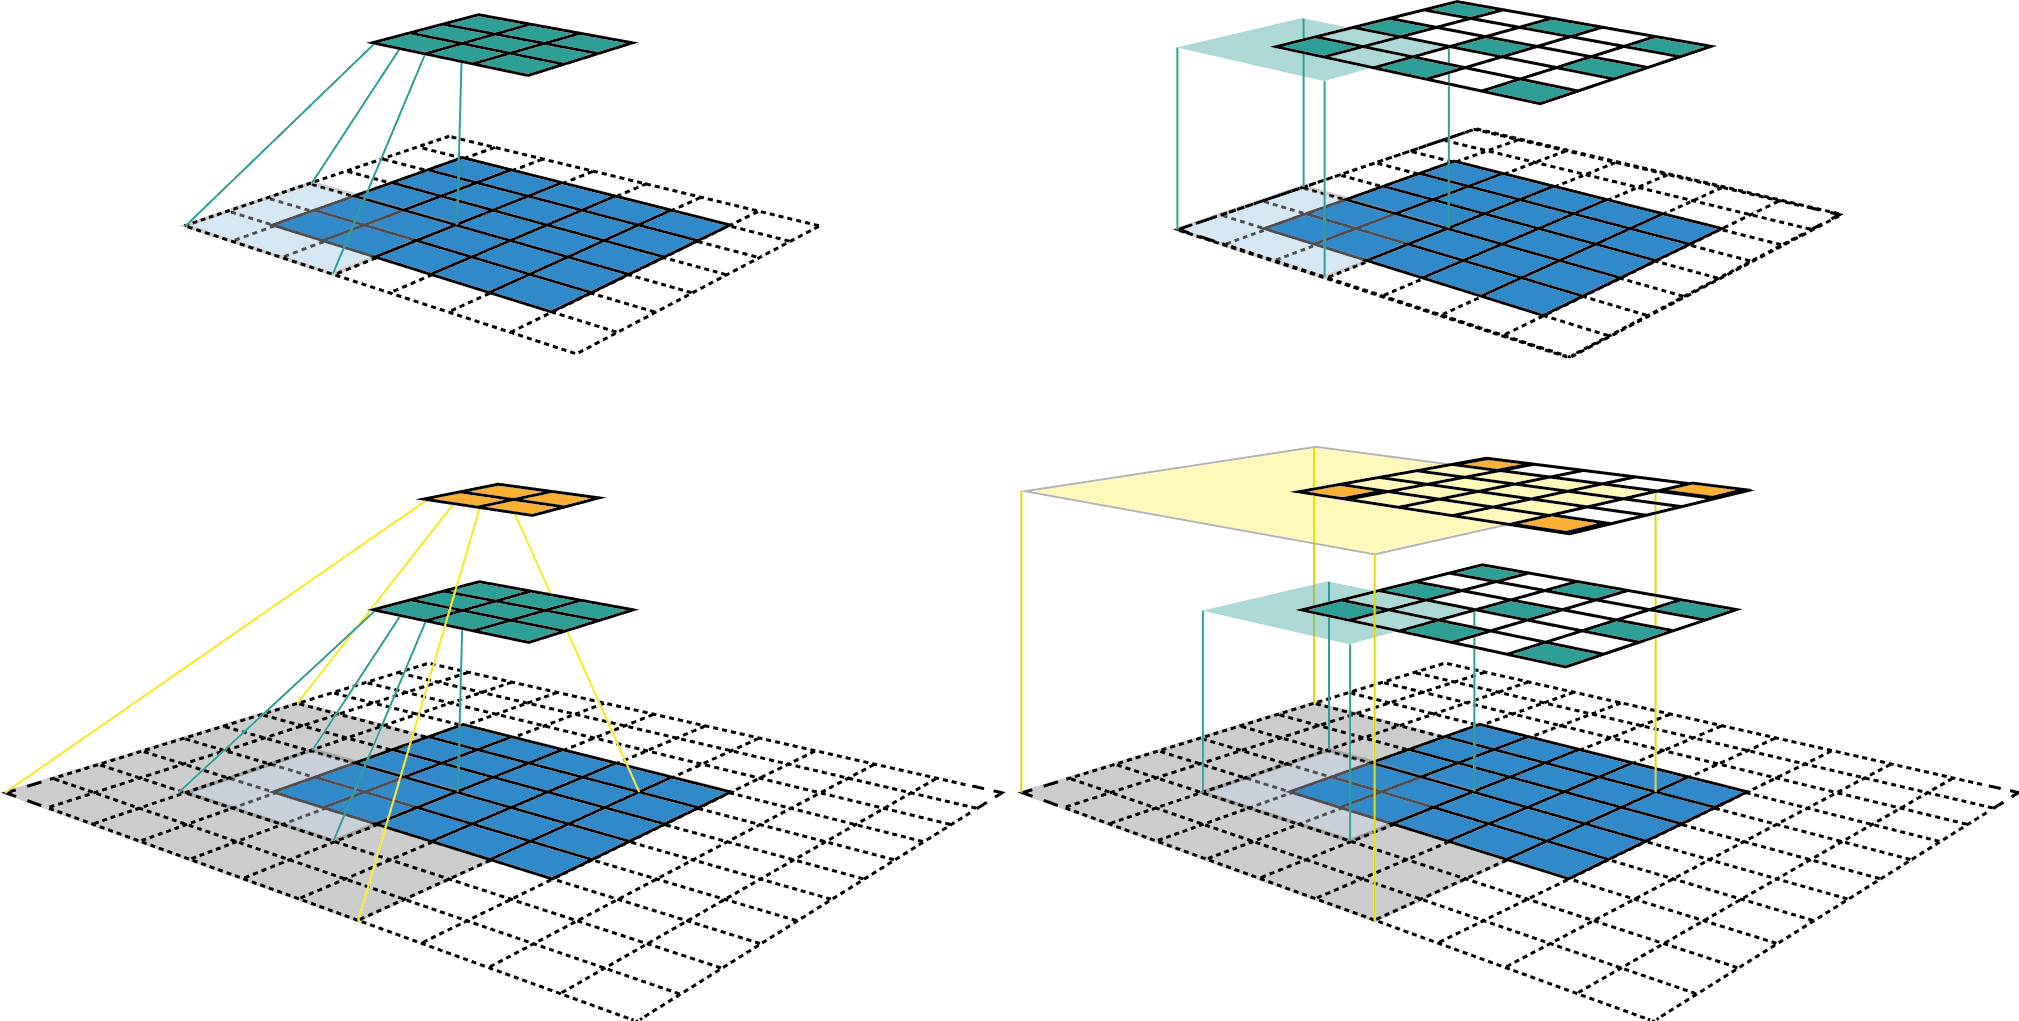
\includegraphics[width=0.75\textwidth]{ReceptionField.png}
	\caption{两种可视化感受野的方法\cite{fang2017reception}}
	\label{fig:ReceptionField}
\end{figure*}

\subsection{深度卷积神经网络的特征提取技术}
\label{subsec:factsdeepextract}
%	Good performance in Classification -> better performance
之所以认为神经网络具有很强的特征提取能力,是因为将在图像分类任务中训练得到的网络参数迁移到解决其他图像任务的网络模型中可以更好地引导网络得到更好的结果\cite{mishkin2015all}。同时根据Yosinski, Jason等人的工作\cite{yosinski2015understanding},在可视化结果中,的确可以看到在分类标签监督下的网络参数对具有语意的区域有较强的响应。所以,大部分希望提高网络特征提取能力的方法都会把目光聚焦在图像分类这一视觉基础任务上。因为在分类任务上更好的性能就意味着网络在特征提取上更强的鲁棒性。

He, Kaiming等人在2015年提出了残差网络\footnote{残差网络,Residual Network,通常被称为ResNet。并且根据具体的层数来分别称呼同种方法的不同的结构,例如101层的残差网络,会被称作ResNet-101。}结构\cite{He2015Deep}。如图\ref{fig:Resblock},文章提出了带有跳跃连接残差模块,将梯度跨层传入浅层的网络,改善了在试图构建深度网络时出现的收敛问题,比如在使用类似VGG网络\cite{simonyan2014very}的策略扩大网络深度时遇到的梯度消失问题。同时,为了减少极大值池化层带来的特征损失,残差网络在下降特征图尺寸时使用了步长为2的卷积层。通过堆叠普通残差模块或瓶颈残差模块,网络能够获得比之前简单堆叠卷积层的策略更加好的分类准确度,和更加稳定的收敛结果。

\begin{figure*}[htbp]	
	\centering
	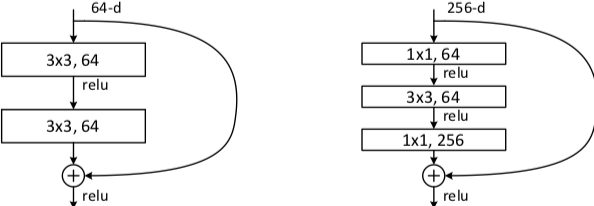
\includegraphics[width=0.6\textwidth]{ResBlock.png}
	\caption{残差模块结构:左图为普通残差模块,右图为瓶颈残差模块}
	\label{fig:Resblock}
\end{figure*}

在残差网络初始的结构策略中,残差薄块可以最多堆叠至152层,如图\ref{fig:ResNet}所示。残差模块的出现让更深层次的网络成为了可能,甚至于在竞赛中出现了千层以上的残差网络。

\begin{figure*}[htbp]	
	\centering
	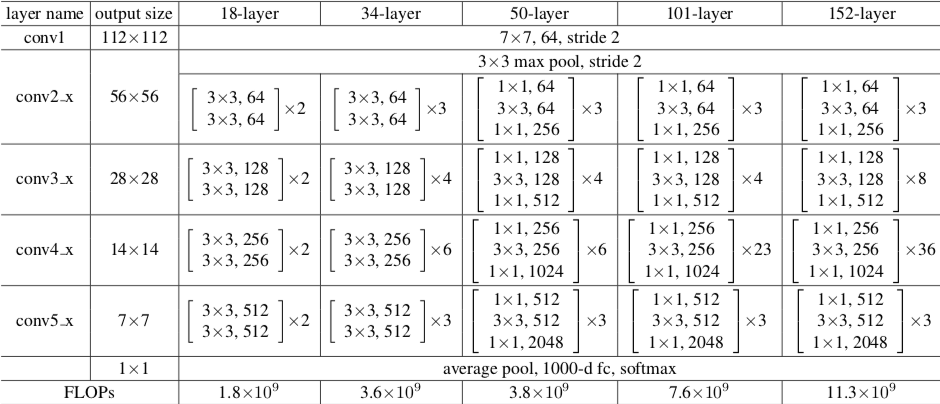
\includegraphics[width=0.9\textwidth]{ResNet.png}
	\caption{残差网络结构策略}
	\label{fig:ResNet}
\end{figure*}

利用残差模块构建深层卷积神经网络来提取特征已经成为了现在使用卷积神经网络的方法普遍做法。残差网络易收敛,大感受野的良好特性让其在各种任务重都能够起到相当重要的作用。

\section{基于深度学习的目标检测方法}
\label{sec:factsobjectdetection}
目标检测对于自顶向下的多人姿态提取而言是十分重要的。由于本文中也使用了一些基于深度学习的目标检测技术,因此在本节简短介绍一下目标检测的相关技术。

\subsection{锚点与检测框}
\label{subsec:factsanchors}
在一些使用卷积网络的目标检测初期方法中,坐标由四个独立的全连接神经元回归而成,如图\ref{fig:MultiBox}左所示。虽然这种方式的确能够回归单个检测框,然而却不能回归出多个检测框。因此,锚点的概念就油然而生。

为了让网络能够在一张图中检测到多个检测框,1\times1卷积层替换掉了传统的全连接层,用来回归分类结果、横纵坐标的偏移量与长宽尺寸的偏移量,如图\ref{fig:MultiBox}右所示。与单检测框方法直接回归坐标不同,多检测框方法中的输出张量中每一个像素位置代表一个检测框,因此这些像素位置本身就包含着类别标签、坐标与尺寸信息。这些像素位置都被称作锚点,使用类别标签来确定候选框的位置,之后经过回归的对应像素位置上的坐标与尺寸偏移量会与锚点所属的坐标与尺寸结合,得到最后的检测框。

\begin{figure*}[htbp]	
	\centering
	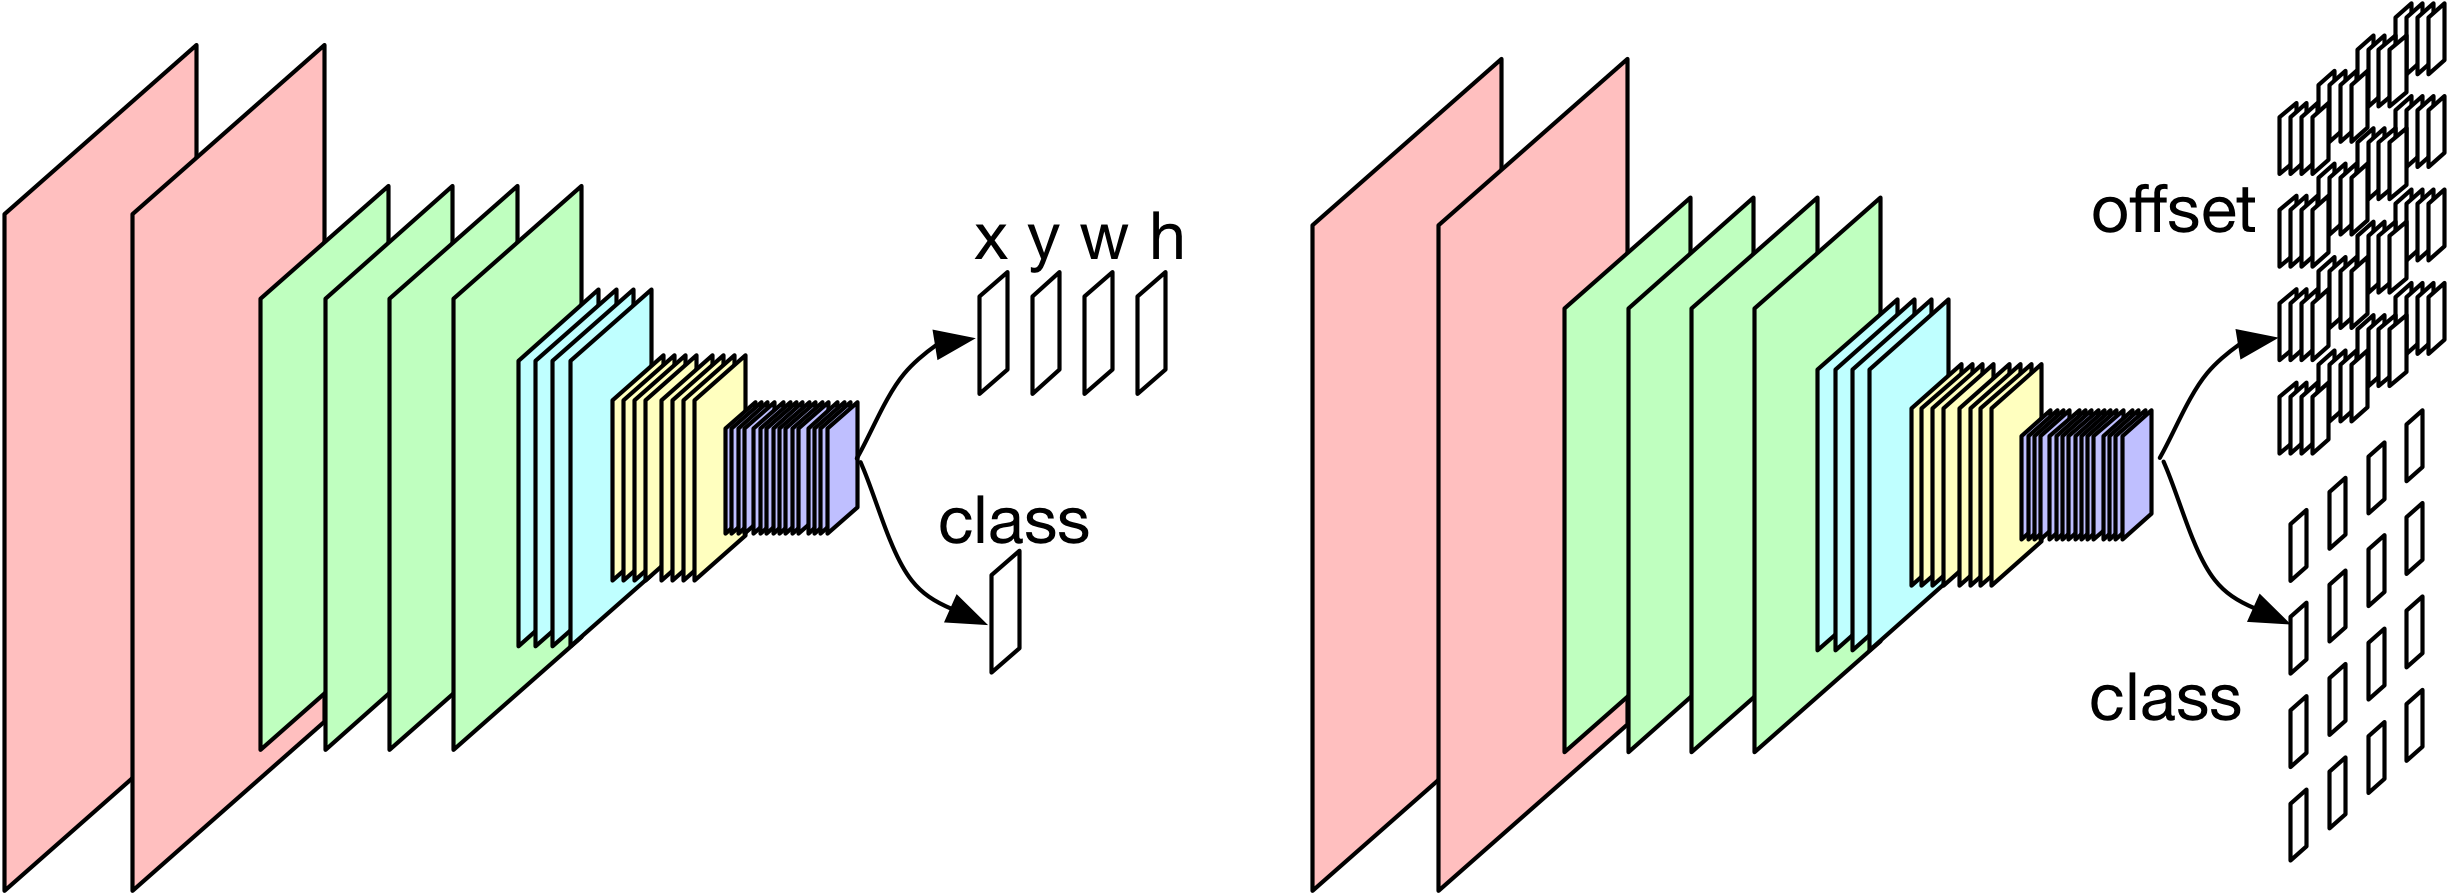
\includegraphics[width=0.7\textwidth]{Anchors.png}
	\caption{基于卷积神经网络的单检测框(左)与多检测框(右)方法}
	\label{fig:MultiBox}
\end{figure*}

\subsection{区域建议网络与回归分支}
\label{subsec:factsRPNregression}
目标检测任务不光要求算法给出检测框结果,同时要给出分类结果。对于每一个检测框算法都需要给出一个类别标签。为了继续保持如图\ref{fig:MultiBox}左中的单检测框方法的结构,一些方法,比如Faster R-CNN\cite{Ren2015Faster},将网络分为两个阶段:在第一阶段中,使用类似图\ref{fig:MultiBox}右的结构,在文章中被称作区域建议网络\footnote{区域建议网络,Region Proposal Network},仅对物体进行前背景分类,并且使用较为贪婪的策略寻找可能是物体的检测框;第二阶段中,网络使用类似图\ref{fig:MultiBox}左所示的结构,将裁剪后的特征送入全连接层对物体分类并对偏移量进行第二次回归。但值得一提的是,一些单阶段的检测器,就是仅使用图\ref{fig:MultiBox}右结构的检测器也可以给出较为精确的结果。不过由于漏检率稍高,单阶段检测器从性能上并不能完全压制两阶段的检测方法。

\section{基于深度学习的多人姿态估计方法}
\label{sec:factspose}
相比目标检测,多人姿态估计的方法更加要求精度。同时,为了考量人体姿态中结构化的信息,网络还需要更多的感受野来对姿态结构进行学习。因此如何以张量形式定义关键点信息与如何监督深度网络成为了姿态估计方法中的两个非常重要的技术。

\subsection{关键点与热图}
\label{subsec:factsheatmaps}
关键点信息与一般的坐标回归不同,其响应对应的区域更小。目标检测中一个锚点对应的是一个物体,也就是至少十余像素边长的范围。但在关键点则不同,一个关键点对应的躯干部位至多几像素大小。对于这样小的区域,如果使用目标检测中的回归锚点位置与偏移量的方法进行学习,是很难让让网络给出鲁棒的响应的。因此常见的关键点表示方法一般是使用多张热图组成的张量共同描述不同关键点的位置。张量中每一通道的热图都表示一类关键点出现的概率,其中单张热图中预测概率的极高值就是网络最终输出的结果。在自顶向上的方法中,一般仅取热图中的最大值作为结果,然而对于自底向下则需要提取更多的关键点。并且在提取更多关键点的时候,要使用极大值抑制来限制过近的位置对其他区域极值点的竞争。

这里有一个很明显的问题:关键点热图的分辨率可能影响最终姿态估计精度。那么为了解决这一点,多数方法故意不使用使用二值响应或标签作为训练数据,而是使用了高斯分布来描述关键点的位置信息。这意味着,在这种监督下,网络在这样的标注数据下将倾向于在关键点的周围生成一些环境响应。这些环境响应并不是没有作用,而是在后处理中,被用于帮助算法通过双线性差值的方式寻找重新映射为真值尺度下的关键点坐标。这样能够较为较为有效地改善低分辨率热图影响姿态估计网络精度的问题。

\subsection{中继监督}
\label{subsec:factsintersupervision}
由于姿态估计算法需要完整考虑人体关键点之间的结构,同时对结果的精度要求也很高,所以相比其他任务而言对感受野大小的要求更为严格。在设计姿态估计网络时,许多工作都是通过增加网络深度的方式来扩大感受野。在监督过深的神经网络时,正如\ref{subsec:factsdeepextract}节中所描述时,会遇到梯度消失的问题而导致过深的网络在性能上出现退化的现象。在Wei, Shih-En等人的工作中\cite{wei2016convolutional}首次提出了中继监督的技巧。中继监督主要是通过将网络切分成完全一致的多个阶段,在每阶段的顶端都加入相同的监督信息约束网络生成相似的结果。这样的技巧主要是旨在解决过深网络中出现的梯度消失问题。中继监督的确能够很好地解决多人姿态中出现的收敛问题,因此这一技术已经成为了现有姿态估计方法中定会采用的监督策略。

\section{本章小结}
本章简略介绍了与多人姿态估计相关的技术。首先,本章由特征提取器的简介开始,说明了特征提取器以及感受野对于网络设计的影响。紧接本章通过对比单检测框与多检测框的检测方法解释了锚点在目标检测的重要性。最后,本章通过阐述关键点回归与边界框回归任务的不同解释了热图在关键点回归中的必要性,同时简略介绍了中继监督的目的与方法。

\chapter{基于弱监督注意力的多人姿态估计方法}
\label{cha:method}

\section{概述}
\label{sec:methodoverview}
%   This part intends to state the overall idea
本方法使用基于残差网络\footnote{残差网络,简称ResNet, 全称Residual Network}与特征金字塔网络\footnote{特征金字塔网络,简称FPN, 全程Feature Pyramid Network}结构的网络框架作为特征提取的骨架,为模型提供各个尺度的特征图。在特征提取部分之后,网络可以分为目标检测与姿态估计和融合回归两个步骤。在目标检测与姿态估计过程中,网络预测出目标的边界框,粗略的关键点预测和实例分割结果。而在融合回归部分,网络会接受从目标检测与姿态估计阶段产生的结果并将它们一同以一定的方式互相交汇并一起回归。而且,在融合回归的过程中,网络采取了多阶段的堆叠和中继监督的策略来共同精炼关键点与实例分割的结果。这种结构是受到CPM\cite{wei2016convolutional}的启发而设计的。同时,为了有效地融合实例分割与姿态估计的结果,网络使用了注意力机制,使其根据实例分割的生成注意力关注网络对应的区域,从而达到方法最初设计的目的,也就是解决多人检测下姿态遮挡的问题。同时,考虑到姿态估计的信息对实例分割也有促进作用,我们设计了双流的网络结构让模型在每个阶段都能同时预测分割结果和姿态估计结果,并送入下一阶段继续优化。网络的整体结果如图\ref{fig:Overall}

%	ROI Extraction
%	key-point & Mask Prdiction
%		Stage One's Prediction
网络通过特征提取器$E$得到图像$I$来自网络各个尺度的特征$F=\{f_1, f_2, ..., f_5\}$。这些特征被兴趣区域对齐层\footnote{兴趣区域对齐层,简称RoI Align Layer, 全称Region of Interest Align Layer}通过双线性插值的方法调整到了同样的尺寸。每个图像中只有来自特定尺度$k$的特征图$f_k$被选中并被输入至接下来的目标检测与姿态估计部分。这个被选中的特征被分别送入了目标检测分支$D$与姿态估计分支$P$,分别得到了实例分割结果$S_1=\{s_1^1, s_1^2, ..., s_1^n\}$与姿态估计结果$K_1=\{k_1^1, k_2^1, ..., k_1^n\}$。这些中间结果会被输入到融合优化阶段进行多阶段的回归。

\begin{figure*}[htbp]	
	\centering
	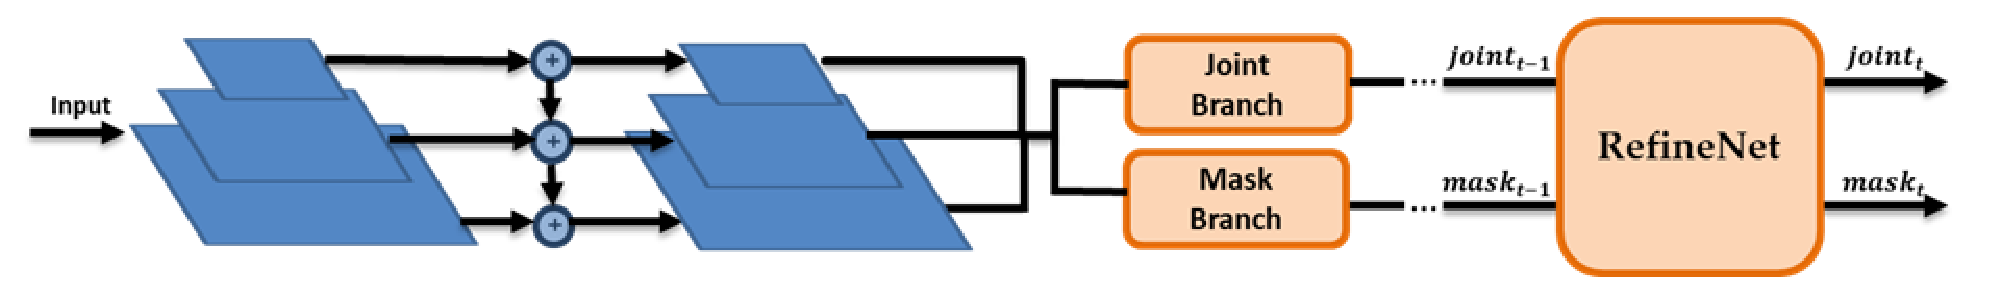
\includegraphics[scale=0.4]{network.eps}
	\caption{网络整体结构}
	\label{fig:Overall}
\end{figure*}

%		Stage 2+'s Prediction
如图\ref{fig:RefineNet}所示,在融合优化阶段的第$t(t>2)$阶段,单个优化模块接收来自特征提取器$E$的特征$f_k$、在阶段$t-1$中得到的姿态估计结果$K_{t-1}$与实例分割结果$S_{t-1}$。整个网络有主要设计亮点可以归纳为三点。第一是我们引入了注意力机制让网络关注具体的区域,我们设计了\textit{Attention Converter}来让生成一个合适的注意力与特征图融合,最后得到关键点预测结果$K_t$。第二,网络还会根据姿态估计的中间结果,也就是一些更偏向于得到关键点预测的特征,生成实例分割的结果。这让网络会根据来自姿态估计的信息修正实例分割的结果。最后,由\textit{Attention Converter}生成的注意力还会与从姿态估计那一支生成的中间结果融合,最终生成的实例分割的优化结果$S_t$。因此,整个优化模块$R$可以被抽象为形如公式\eqref{def:refinenet}的函数。


\begin{equation}
\label{def:refinenet}
M_t, K_t = R(M_{t-1}, K_{t-1})
\end{equation}

%   This part is to describe why we use a hybrid multi-stage arch
%	1. mask and key-point detection is associated
%	2. In crowd, the heatmap is not robust to predict
本方法使用了多阶段、利用弱监督约束的注意力的结构,同时优化实例分割与姿态估计的结果。首先多阶段与中继监督这两个设计可以让网络获得更大的感受野,让网络能够充分学习关键点之间的关系\cite{wei2016convolutional}。其次,由于实例分割和姿态估计是联系紧密的两个任务, 正如本文\ref{sec:generalmotivation}中提到的,实例分割与姿态估计能够相互优化,并且有相当大的相关性。所以这样设计的结构主要是希望能够同时优化姿态估计与实例分割结果。通过引入注意力以及弱监督这种较宽松约束下的可学习参数,网络能够更加适应数据中的不同表现。这让网络在一些实例分割无法正确引导关键点检测的情况下, 仍然能够生成较为正确的注意力引导关键点的检测与人体骨架的重建。

\begin{figure*}[htbp]	
	\centering
	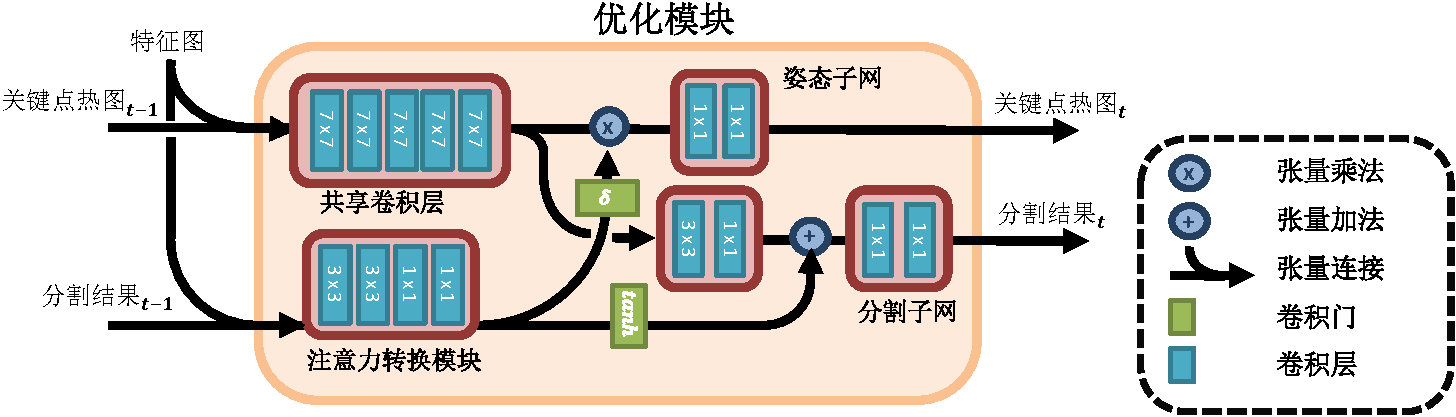
\includegraphics[scale=0.65]{RefineNet.pdf}
	\caption{融合优化模块具体设计}
	\label{fig:RefineNet}
\end{figure*}

\section{目标检测与姿态估计}
\label{sec:detectionstage}
%	Structure description
%	1. Hybrid arch of maskrcnn & cpm
本文在特征提取部分使用了101层的残差网络与特征金字塔网络来生成不同尺度的特征图供检测部分使用。正如Mask R-CNN\cite{He2017Mask}中使用的结构,本文也设计了并行的区域建议网络,在经过回归分支后从不同尺度的特征图上得到来自不同尺度的边界框。这些尺度不同的边界框会根据其来源送入专为特征金字塔网络设计的兴趣区域对齐层,根据公式选定对应的层数来裁剪并对齐特征图\cite{Lin2016Feature}。这样裁剪下来的特征图具有相对平衡的感受野:小尺寸物体有较小的感受野大小,同时大尺寸物体会获得更大的感受野大小。

检测部分是由两个并行的分支组成的。实例分割与姿态估计分支分别使用裁剪好的特征得到粗略的实例分割结果与姿态估计结果。分割分支的网络结构使用了四层卷积核大小为3像素的卷积层,和一层步长为2,卷积核大小为2的空洞卷积层。同样的,姿态估计分支使用了五层卷积核大小为3的卷积层,最终的输出被两层1x1卷积调整至关键点外加背景个通道,以得到每个关键点的热力图。


%   Training strategy description
%	Section 1
在检测部分的监督过程中,由于我们将网络设计为能够完成两个任务的并行的分支,所以该部分的损失函数设计就表现为两个损失函数加和的形式,如公式\eqref{detection_loss}所示。首先我们需要对目标位置检测进行监督,所以我们就借鉴区域卷积神经网络\cite{Girshick_2014_CVPR}中损失函数设计思路,使用交叉熵来计算预测标签与真实标签之间的距离。同样的,如Mask R-CNN\cite{He2017Mask}中的损失函数设计,交叉熵也被用来监督实例分割。公式\eqref{bbox_mask_loss}描述目标检测与实例分割的损失函数设计。姿态估计分支的损失函数被定义为均方差的形式,如公式\eqref{coarse_key-point_loss}所示。

\begin{equation}
%	section 1 loss
\label{detection_loss}
L_{detection} = L_{bbox\&mask_{reg}} + L_{key-point_{reg}}
\end{equation}      
\begin{equation}
%	bbox & mask regression loss
\label{bbox_mask_loss}
L_{bbox\&mask_{reg}} = -\sum_{c \in C}{\hat{p_c} \log{p_c^{*}}}  -\sum_{c \in C}{\hat{m_c} \log{m_c^{*}}}
\end{equation}
\begin{equation}
%	coarse mask regression loss
\label{coarse_key-point_loss}
L_{key-point_{reg}} = -\sum_{i \in I}\sum_{k \in K}{\left\| \hat{k_i} - {k_i}^{*} \right\|_2}
\end{equation}


\section{融合优化}
\label{sec:refine}
\subsection{网络结构}
\label{subsec:architecture}
%	TODO: more detailed content to discuss the net structure in refine section
%	1. What the network looks like
%	2. Why we propose the network like this? (need to be explain by experiments)
%		a) training process (featured points)
%			(i)		loss penalty calculation
%		b) inference process 
%			(i)		attention-like instance segmentation
%Size of reception field is crucial to the refine section, as the key-point branch need them to avoiding the wrong decision in 
融合优化阶段由数个完全一样的优化模块组成,每个模块可以被抽象地定义为公式\eqref{def:refinenet}。
% TODO: bookmark in chapter 03

The refine section is divided into 5 seperated stages, and each part can be denoted as equation\eqref{def:refinenet}, to be more in detail, the network can be defined as below:
\begin{equation}
c = C({f}\otimes{K_{t-1}})
\end{equation}
\begin{equation}
a = A(f\otimes{M_{t-1}})
\end{equation}
\begin{equation}
K_t = H_k(c\odot a)
\end{equation}
\begin{equation}
M_t = H_m(F(c) \oplus a)
\end{equation}
第一份拷贝会首先与来自阶段$t-1$的姿态结果$K_{t-1}$进行合并,并一同被送入一组\textit{Shared Convolution Layers}中。第二份拷贝同样会与上一阶段的实例分割结果$S_{t-1}$进行合并,并被输入至\textit{Attention Converter}中。经过\textit{Shared Convolution Layers}的特征图会与\textit{Attention Converter}中$\sigma$门生成的注意力热图相乘。最终输出对关键点估计优化的结果$K_t$。同时\textit{Shared Convolution Layers}的特征图的另一份拷贝在经过两层卷积层后,会与\textit{Attention Converter}中$\tanh$门的输出相加,输出对实例分割的优化结果$S_t$。

where $\otimes$ refers to concatenating operation, $\odot$ for bit-wise multiply, and $\oplus$ is for bit-wise add operation. $M_t$ and $K_T$ denote the mask and key-point prediction from stage $t$. The feature map is denoted as $f$, and $a$ is for attention, $c$ is for the output from the shared convolution layers. In notations for modules, $C$ is for shared convolution layers, $A$ is for attention converter, and $F$ is for the fusion module. $H_k$ is for the key-point head, and the $H_m$ is for mask head.\\
It is common to generate attention using a given feature from last stage, and we suppose that the instance segmentation prediction, still can be treated as a strong cue to the soft attention. Therefore, our method proposed a attention converter to digest features and mask prediction from last stage to generate proper attention to the network.\\
However, the attention may be incompatible for a multi-staged architecture to supervise. Hence, a single layered mask head is designed here to adjust the dimension to the binary mask, which makes it easier to define losses to the attention. In another hand, like other the traditional multi-tasking networks, our method also employs a separated head which accepts features from a shared convolution to use the common priors which are used by the key-point prediction. To hybrid those two idea in the design of networks, we proposed the refine stage which is shown in Fig.\ref{fig:RefineNet}.\\

\subsection{损失函数定义}
\label{subsec:lossfunctions}
%	Section 2 Training
%	key-point Loss
%	Why Applying masks after 1x1 conv?
%	1.	explicitly define loss with mask & key-points
%	2.	simply enhance response of the heatmap
%		rather than enhance the result
%			--> This will give more responses
%	TODO: quote attention paper to prove it
Training strategy in section 2 is divided into two parts: key-point branch loss and instance segmentation loss. Loss in section 2 can be defined as a summing function from the second stage to the last \eqref{total_refine_loss}, where $\alpha$ is 0.05.

%	TODO: fit the <Attention is all you need> thread into this section
Training key-point branch is similar to the process in section 1. We define MSE loss to measure errors between ground truth and prediction. But what is different in section 2 is that the key-point predictions are affected by the instance mask implicitly, as we multiply them with those masks in a bit-wise fashion before 1x1 convolution layers. The 1x1 convolution layers will not change the size of reception field, therefore the operation we perform here are nearly the same as multiplying after the network. But with those trainable parameters in 1x1 convolution layers, the network will need no explicit definition of any masks in loss function of the key-point branch and also can strengthen the response at relative positions on feature maps. This is intended to avoid multiplying zeros on the result in key-point branch, which causes failure on supervising both key-point prediction and instance segmentation with one loss. The loss function in key-point branch $L_{k_t}$ where $t>1$ is defined as \eqref{refine_key-point_loss}. 

%	Total Refine Loss
\begin{equation}
\label{total_refine_loss}
L_{refine} = \sum_{t=2}^{T}{L_{k_t} + \alpha L_{m_t}}
\end{equation}

%	Refine key-point Loss
\begin{equation}
\label{refine_key-point_loss}
L_{k_{t}} = -\sum_{i \in I}\sum_{j \in J}{\parallel \hat{k_i} - {k_i}^{*} \parallel_2}
\end{equation}

%	Instance segmentation supervision
%	Localization loss
%		smoothed L1
%			attention-like
%	TODO: More attention paper quotations
Supervising mask branch is a more complicated process, because we want to train the network in order to complete the losing part where the detection section failed to infer. Therefore we consider to calculate both localization error and overlap penalty \eqref{mask_loss} for stage $t$ where $t>1$. We set the $beta$ in equation\eqref{mask_loss} to 0.2. The localization error is defined as \eqref{mask_loc_loss}. Instead applying a cross entropy loss here, we introduce smoothed L1 loss here, as the network use instance segmentation as attention.

%	Mask Loss
%	Semi supervision
\begin{equation}
\label{mask_loss}
L_{m_t}=L_{loc_t} - \beta L_{ins\ penalty_t}
\end{equation}

\begin{equation}
\label{mask_loc_loss}
L_{loc}^t =  \sum_{p \in P} Smooth_{L1}( H^{p}_{gt} - H^{p}_{pred} )
\end{equation}

\subsection{训练策略}
\label{subsec:trainingstrategy}
%	TODO: Training Strategy
%	Training Setups
%		learning rate
%		optimizer
%		separated trained ( sec 1 -> sec 2)
We use a two-stage separated training strategy. In the first stage, we train the joint branch only at learning rate of 4e-4 (all stages) for 60 epochs, with the epoch size of 1000 and the exponential learning rate decay (0.333 every 20 epoch). In the second stage, we train the whole refine branch with the total Loss, which equals to refine joint loss plus refine mask loss multiply by ten, with the base lr 1e-4 with exponential decay of 0.333 every 30 epoch.


\begin{figure}[htbp]
	\centering
	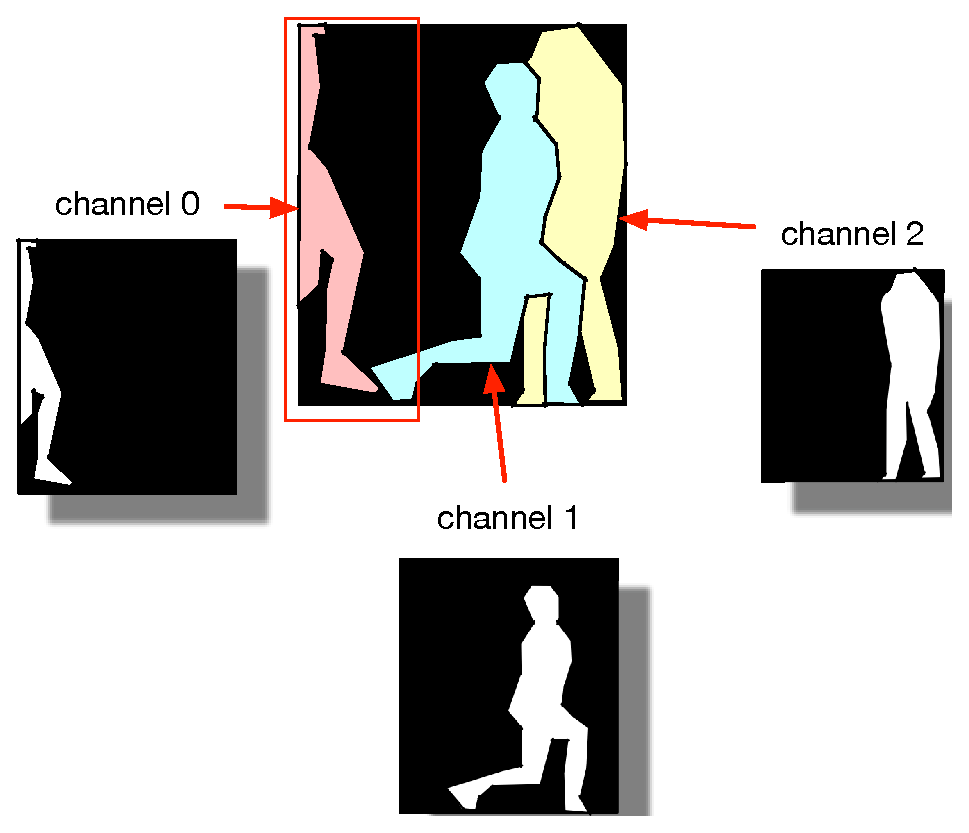
\includegraphics[scale=0.34]{instance_segmentation.eps}
	\caption{Channel-wise instance segmentation}
	\label{fig:chInsSeg}
\end{figure}

\section{本章小结}

\chapter{实验验证与分析}
\label{cha:exp}
在实验中,我们在COCO2017验证数据集上达成了46.7mAP的姿态检测结果,证明了本文中的优化模块的确优化了多人姿态估计网络的性能。同时,为了证明方法的有效性,我们完成了一些实验来证明我们提出的弱监督下的注意力以及其对应的网络结构能够较好地在解决多人遮挡的问题的同时,改善关键点与实例分割的结果。
\section{数据集与评价指标}
\label{sec:dataset}
为了验证在\ref{sec:refine}节中提出的网络结构,本文设计了使用mAP作为评价指标的消融实验与性能对比实验。在实验中我们使用了COCO2017验证数据集\cite{lin2014microsoft}作为我们验证的数据集。平均准确度(mAP,mean Average Precision)\cite{zhu2004recall}指标都是旨在统计一定容忍度下的关键点命中情况。平均准确度通过计算交并比(IoU, Intersection over Union)来求得不同物体关键点相似度(OKS,Object Key-point Similarity)\footnote{物体关键点相似度从0.5取值至0.95,间隔为0.01。}下的准确率,并对这些准确率进行积分得到最终平均准确率。

\begin{figure}
	\centering
	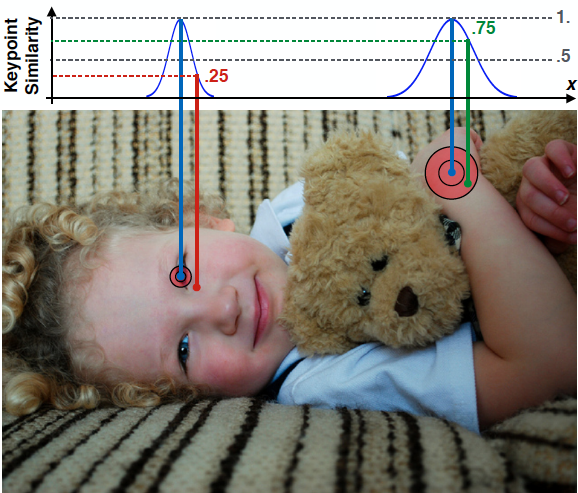
\includegraphics[width=0.6\linewidth]{OKS.png}
	\caption{物体关键点相似度图示\cite{ruggero2017benchmarking}}
	\label{fig:oksfigure}
\end{figure}

物体关键点在计算交并比的时候,需要设置关键点的容许度半径,如图\ref{fig:oksfigure}中所示。不同的关键点拥有不同的容许度半径。比如眼睛的容许度半径一定比手腕的容许度范围要小。在图\ref{fig:oksfigure}中,手腕与眼睛的预测关键点与真值的距离相当,然而给出的命中判定却不相同。因为人类对眼睛关键点的标注方差更小,对手腕关键点的标注方差更大。COCO数据集根据人类对于不同关键点标注的方差大小设置容许度半径来判别关键点命中是合理的。这比一些通过标准化距离阈值来判别命中的方法,比如关键点命中概率曲线\cite{andriluka20142d}(PCK,Probability of Correct Key-point)更加科学。

\section{性能对比}
\label{sec:perfcompare}
本节中文章主要通过对比网络在mAP指标上的表现,来对比网络与现有方法的性能。在对比的同时还会给出结果分析,尝试从实验结果验证网络结构设计的优势。本文选取了自顶向下结构的堆叠沙漏模型作为我们的对比方法。
% TODO: 比较表格
\begin{table*}[ht]
	\centering
	\caption{COCO公开测试集的模型性能对比}
	\label{tab:mAPCOCObenchmark}
	\begin{minipage}[t]{0.8\linewidth}
		\begin{tabular}{p{0.25\linewidth}p{0.1\linewidth}<{\centering}p{0.1\linewidth}<{\centering}p{0.1\linewidth}<{\centering}p{0.1\linewidth}<{\centering}p{0.1\linewidth}<{\centering}}
			\hline
			方法 & \multicolumn{1}{c}{$mAP$} & \multicolumn{1}{c}{$AP_{OKS=0.5}$} & \multicolumn{1}{c}{$AP_{OKS=0.75}$}
			& \multicolumn{1}{c}{$AP_M$} & \multicolumn{1}{c}{$AP_L$} \\
			
			& \multicolumn{1}{c}{(\%)}& \multicolumn{1}{c}{(\%)}&
			\multicolumn{1}{c}{(\%)}& \multicolumn{1}{c}{(\%)}& \multicolumn{1}{c}{
				(\%)}\\
			\hline
			Top-down SHN\cite{newell2016stacked} & 46.0 & 74.6 & \textbf{48.4} & 38.8  & \textbf{55.6} \\
			本文复现 & 41.2 & 71.3 & 45.9 & 34.2 & 47.4 \\
			本文方法$^1$ & 45.9 & 82.1 & 45.3 & 43.0 & 51.6 \\
			本文方法+ $^2$ & \textbf{46.7} & \textbf{83.4} & 46.6 & \textbf{45.1} & 53.2 \\
			\hline
		\end{tabular}\\[2pt]
		\noindent\rule{0.25\linewidth}{1pt} \\
		\footnotesize
		1: 使用直接连接的4个堆叠的优化模块,在本文提出的整体训练策略下收敛的模型。\\
		2: 使用2个$7\times7$组成的回归模块和4个堆叠的优化模块,在本文提出的整体训练策略下收敛的模型。
	\end{minipage}
\end{table*}

在表\ref{tab:mAPCOCObenchmark}中,可以明显看到本文在宽松条件下(OKS=0.5)的关键点准确度明显优于本文复现的自顶向下框架和SHN网络的结果。这一结果要归功于网络中使用弱监督学习方法监督的注意力机制,其生成的关注区域帮助网络生成更加紧凑的关键点结果。同时在小目标检测\footnote{在COCO数据集中,小目标通常指边界框面积小于$64^2$的目标。}中明显优于传统的自顶向下的方法。虽然在更高精度下的指标比SHN略差,但是差别并不明显,同时在整体的指标,也就是积分得到的平均准确度中,能够比SHN的性能更优。

% TODO: 计算量对比


\section{消融实验与分析}
\label{sec:ablation}
本节中文章设计了消融实验验证优化模块的作用以及有效性。本文提出了多种消融策略来控制优化模块中不同部件出现,从而通过量化指标和可视化效果来量化优化模块对提高算法性能的贡献。
\subsection{消融策略}
\label{subsec:selfstrategy}
由于本文提出了一种能够融合实例分割信息的新结构,因此需要设计自对比实验来证明文章提出的结构能够改善基线方法
本文设计了三种自对比的网络结构策略:
\begin{itemize}
	\item \textbf{单任务无融合}:不使用多任务分支的简单结构也不使用注意力机制的网络结构。
	\item \textbf{多任务无融合}:使用多任务分支但不使用注意力机制的网络结构\footnote{多任务分支指加入实例分割任务训练,但不使用注意力交叉与传递特征信息。}。
	\item \textbf{多任务融合}:使用多任务分支且使用注意力机制的网络结构。
	\item \textbf{多任务融合}:使用多任务分支且使用注意力机制的网络结构,并使用更多的堆叠的网络模块。
\end{itemize}

\subsection{消融性能实验}
\label{subsec:selfeval}

本文根据\ref{subsec:selfstrategy}节中提到的消融策略完成了在COCO数据集上的消融性能实验。实验结果如表\ref{tab:mAPCOCOselfbenchmark}所示。

% TODO: 自对比表格数据填充
\begin{table}[ht]
	\centering
	\caption{自对比mAP评价数据}
	\label{tab:mAPCOCOselfbenchmark}
	\begin{minipage}{0.8\linewidth}
		\begin{tabular}{p{0.25\linewidth}p{0.1\linewidth}<{\centering}p{0.1\linewidth}<{\centering}p{0.1\linewidth}<{\centering}p{0.1\linewidth}<{\centering}p{0.1\linewidth}<{\centering}}
			\hline
			方法 & \multicolumn{1}{c}{$mAP$} & \multicolumn{1}{c}{$AP_{OKS=0.5}$} & \multicolumn{1}{c}{$AP_{OKS=0.75}$} 
			& \multicolumn{1}{c}{$AP_M$} & \multicolumn{1}{c}{$AP_L$} \\
			
			& \multicolumn{1}{c}{(\%)}& \multicolumn{1}{c}{(\%)}&
			\multicolumn{1}{c}{(\%)}& \multicolumn{1}{c}{(\%)}& \multicolumn{1}{c}{
				(\%)}\\
			\hline
			单任务无融合 & 41.2 & 71.3 & 45.9& 34.2& 47.4\\
			多任务无融合 & 38.8 & 78.4 & 25.6 & 30.1 & 37.7 \\
			多任务有融合 & 45.9 & 82.1 & 45.3 & 43.0 & 51.6 \\
			多任务有融合+ & 46.7 & 83.4 & 46.6 & 45.1 & 53.2 \\
			\hline
		\end{tabular}
	\end{minipage}
\end{table}

表格\ref{tab:mAPCOCOselfbenchmark}描述了本方法在COCO开放验证数据集上的表现情况。其中,单任务无融合策略是这四种策略中的基准,因为其仅仅完成单个关键点定位任务,且没有引入注意力机制。在表\ref{tab:mAPCOCOselfbenchmark}中我们可以看到,多任务无融合的实验结果明显低于我们的基准方法,也就意味着简单将多任务直接使用多分支回归会影响最终关键点定位的精度。可以明显地看到在多任务无融合的策略下,在高精度阈值下的准确率明显下降了。

然而在加入融合,也就是使用空间注意力将两任务连接后,网络在高精度要求下的准确度大幅提升。这是得益于多任务的损失函数可以通过梯度回传至分散的分支以让网络更好地收敛。相比之下,网络能够更好地融合实例分割,让关键点检测的结果比基准方法中给出的有多提高。这证明了使用注意力连接的优化模块比一般的多任务分支网络性能能更好,同时也验证了使用优化模块来加入实例分割信息能够有效改善关键点行为的性能。

\subsection{注意力可视化}
\label{sec:weaksuperatten}
本文将网络中输出的空间注意力可视化,并于原图混合得到了最终可视化的结果。
% TODO: 结果效果图
\label{subsec:attenexp}
\begin{figure*}
	\centering
	\begin{minipage}{\textwidth}
		\centering
		\begin{sideways}
			\begin{minipage}{1cm}
				 \rightline{遮挡人}
			\end{minipage}
		\end{sideways}
		\begin{subfigure}{0.2\linewidth}
		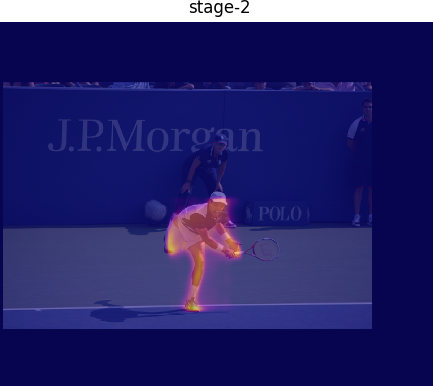
\includegraphics[width=\linewidth]{885_insid0_stage2.PNG}
		\end{subfigure}
		\begin{subfigure}{0.2\linewidth}
		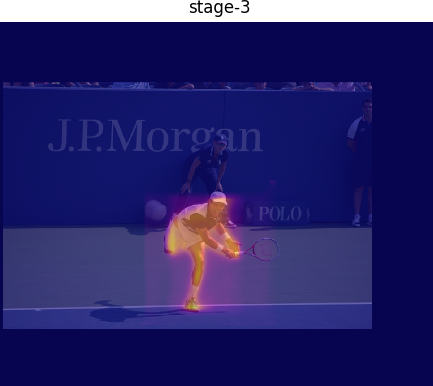
\includegraphics[width=\linewidth]{885_insid0_stage3.PNG}
		\end{subfigure}
		\begin{subfigure}{0.2\linewidth}
		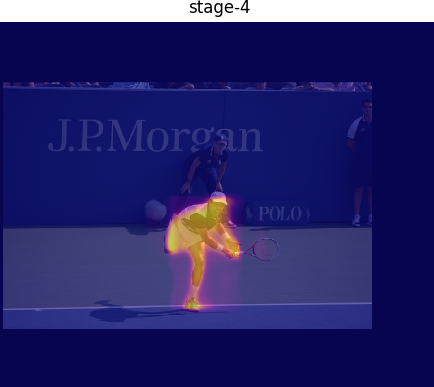
\includegraphics[width=\linewidth]{885_insid0_stage4.PNG}
		\end{subfigure}
	\end{minipage}

	\begin{minipage}{\textwidth}
		\centering
		\begin{sideways}
			\begin{minipage}{1cm}
				\rightline{被遮挡人}
			\end{minipage}
		\end{sideways}
		\begin{subfigure}{0.2\linewidth}
			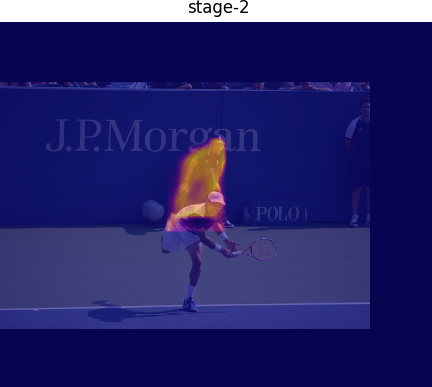
\includegraphics[width=\linewidth]{885_insid1_stage2.PNG}
			\caption{stage 2}
		\end{subfigure}
		\begin{subfigure}{0.2\linewidth}
			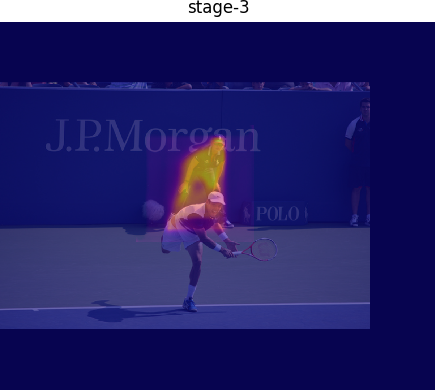
\includegraphics[width=\linewidth]{885_insid1_stage3.PNG}
			\caption{stage 3}
		\end{subfigure}
		\begin{subfigure}{0.2\linewidth}
			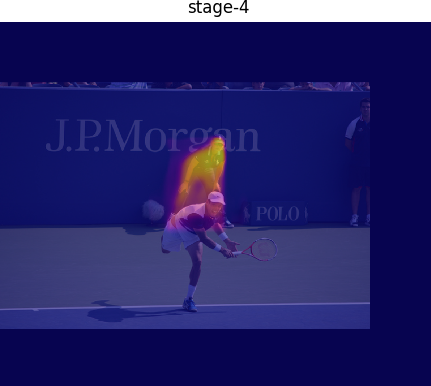
\includegraphics[width=\linewidth]{885_insid1_stage4.PNG}
			\caption{stage 4}
		\end{subfigure}
	\end{minipage}
	\label{fig:parallel1}
	\caption{示例组1}
\end{figure*}


\section{实验效果}
\label{sec:demo}

\section{本章小结}
\begin{conclusion}
多人姿态估计已经在商业应用以及工业场景中体现了极高的价值。本文提出一种全新的可以融合人体实例分割信息的姿态估计网络结构。该结构将实例分割信息加入到多阶段的优化网络设计中,同时优化分割结果与姿态估计结果。实例分割结果可以帮助姿态估计任务寻找网络应该关注的空间区域,并且姿态估计还可以让实例分割根据关键点任务中提取的特征使分割结果更加完整。

本文提出的结构与技术可以被推广到实例分割与关键点定位这两个任务以外的其他任务上。首先,引入注意力机制让网络自主学习关注区域可以结合任务中的监督信息,使用数据驱动的方式让网络自适应训练数据集生成对应的关注区域,提高网络的泛化性;同时本文提出的弱监督学习的训练方法,可以用来训练难以通过显式监督约束的输出的生成。这让网络能够通过其他任务重损失函数的定义监督一个困难任务。

然而本文提出的结构仍然存在一定的缺陷。本文的结构没有充分考虑优化模块中周围注意力的生成,换言之,网络仅仅会自顾自地生成关于一个实例的注意力而不考虑其他实例注意力的生成。如果加入一个全局卷积来考虑整体注意力的生成的话,也许能够改善网络对于更困难情形下遮挡问题的解决能力。

\end{conclusion}


%%% 其它部分
\backmatter

%% 本科生要这几个索引,研究生不要。选择性留下。
% 插图索引
\listoffigures
% 表格索引
\listoftables
% 公式索引
\listofequations


%% 参考文献
% 注意:至少需要引用一篇参考文献,否则下面两行可能引起编译错误。
% 如果不需要参考文献,请将下面两行删除或注释掉。
\bibliographystyle{thuthesis-numeric}      % 顺序编码制
% \bibliographystyle{thuthesis-author-year}  % 著者-出版年制
% \bibliographystyle{thuthesis-bachelor}     % 本科生参考文献的著录格式
\bibliography{ref/refs}


%% 致谢
% 如果使用声明扫描页,将可选参数指定为扫描后的 PDF 文件名,例如:
% \begin{acknowledgement}[scan-statement.pdf]
\begin{acknowledgement}
衷心感谢导师马伟教授对本人的精心指导。老师在完成毕设中提供了相当多的帮助与支持。如果没有马伟老师的辅导,本人一定没有办法顺利完成本人的毕业设计。马老师对于本人的毕业论文非常认真。不论是实验设计上或是文章结构上,老师都会倾心给出建议。同时老师也非常重视学生的看法,每次的课题讨论,老师都会结合同学的想法给出建议。同时本人也非常感激马伟老师对我的器重与支持。老师并没有因为本人是从人文学院转系来而拒绝我的申请,而是给了相当多设备上和科研上的支持。对这些来自老师的帮助本人仅用一次致谢难以平复心情,所以再次向老师致以最衷心的感谢,感谢老师对我的付出以及培养。

同时在中国科学院自动化所进行三个月的实习期间,承蒙徐士彪副教授热心指导与帮助。徐老师在实习结束后仍乐于解答本人的困惑,这让本人在接下来的工作中避免了很多不必要的试错,不胜感激。徐老师在答疑解惑的过程中,也教会了许多科研上的经验,这让我受益匪浅。

对以上两位老师谢意难以言表,故作词:器重之恩难相报,桃李之后定相告。

马伟老师实验室的各位师兄师姐们也给本人提供了相当多的帮助。李曈师兄与郑玛娜师姐在他们实验空余时间将GPU借给本人使用,同时还在休息至于给本人提出了很多有用的建议,这让我不光在进度上有明显的推进,还让我学习了很多前沿领域的知识与技巧。

同时还要感谢本人父母在完成论文时给予的坚实支持。情绪上的稳定与实验进度有着相当大的关系。父母在本人顾及不到之处给了不可缺少的支持,让本人平稳地走过了这相当忙碌的大学四年。所以在论文中必须要感谢父母对本人的理解与关怀,尤其在这大学最后一年中让我专心完成学业。

最后要感谢本人的挚友们。相识的机缘也许不同,但友人们在本人迷茫时给予的关怀是相同的。虽然道路不一样,但是只要一直努力下去,就一定会看到未来。这让我想起了一段话:


{\fangsong {\textbf{“}\erhao}}

\begin{minipage}{0.8\textwidth}
{\fangsong
\hskip2cm没错,我们至今为止所做的一切都不是徒劳的。

\hskip2cm只要我们不止步,前方就会有路....

\hskip2cm所以,不要停下来...}
\end{minipage}

\hfill{\textbf{”}\erhao}

本人也会在毕业之后,继续带着各位给本人的祝福与期望,继续努力下去的。

  
\end{acknowledgement}


%% 附录
\begin{appendix}
\title{《多人区域姿态估计网络》\\ 
	RMPE: Regional multi-person pose estimation\\
	{\wuhao Hao-Shu Fang, Shuqin Xie, Yu-Wing Tai, Cewu Lu}\\
}
\section*{摘要}
在开放场景多人姿态估计是一个非常有挑战的任务。虽然现有的人体检测器已经展现出较好的效果,但是在一些困难场景下检测和识别误差中仍然无法避免。这些误差会导致在多人姿态检测系统系统在单人姿态估计网络阶段产生失误,尤其是一些非常依赖人体检测结果的方法。在本文中,我们提出了一种全新的区域多人姿态估计架构,用于改善人体检测器中可能出现的误差。我们的框架由三部分组成:对称空间变换网络,参数化姿态极大值抑制,以及姿态引导的目标框引导生成器。我们的方法可以应对不准确的检测框,并产生冗余的检测结果,让本方法在MPII数据集上达到76.7mAP的成绩。本文中的模型以及源码已经向公众开放。

\section*{引言}
人体姿态估计是一个计算机视觉领域中主要的挑战。在实践过程中,在开放环境中识别多人姿态要比从数字图像中恢复单人姿态更加有挑战性。近年的一些方法尝试通过两阶段框架,或者是一个基于部件的框架完成该任务。在两阶段的框架中,网络首先检测人体目标的边界框,之后对每一个边界框单独地回归姿态。而基于部件的框架首先检测所有的人体关键点,并根据检测到的人体关键点重新组装生成多个人体姿态。这两类框架都有各自的优点与缺点。对于两阶段框架而言,姿态估计结果高度依赖于人体检测框结果的质量。对于基于部件的框架而言,多人姿态估计结果可能会由于多个相互接近的人体而导致检测结果过于模糊。同时,由于基于部件的框架仅从底层考虑身体部件的结构,因此其难以全局地考量各个身体部位之间的关系。

我们的方法遵从两阶段框架。我们着眼于在不准确的目标检测框下检测精准的人体姿态。为了表现之前方法的缺陷,我们使用了现代检测器Faster R-CNN和用于但人姿态估计的堆叠沙漏网络进行了测试。如图1与图2中所示,一般两阶段的网络面临了一下两种缺陷:定位误差以及冗余检测。实际上,单人姿态估计网络是一个对目标检测结果容忍度很低的网络。即使在考虑交并比大于0.5为检出结果的条件下,单人姿态估计网络得到的单人姿态很有可能还是错误的。因为单人姿态估计网络针对于检测框生成姿态估计结果,一些冗余的检测结果就会得到冗余的姿态估计结果。

为了改善上述问题,本文提出了区域多人姿态估计框架。我们的框架改善了基于单人姿态估计网络的多人姿态估计算法。我们设计了附加在单人姿态估计网络后对称空间变换网络来从不精确的目标检测框中提取高质量的单人人体区域。在本文中,这些单人人体姿态估计网络都是以并行的方式排布在我那个罗中。同样为了消除检测冗余的问题,我们还引入了参数化姿态极大值抑制。我们的参数化姿态极大值抑制使用全新的姿态距离评价来给出姿态相似度,从而消除冗余的姿态估计结果。最后,我们设计了全新的姿态引导的人体检测框生成器来扩增训练样本。通过学习人体检测器对于不同姿态的输出分布,可以模仿检测器生成大量的训练样板。

我们区域多人姿态估计框架可以被迁移至不同的人体检测器与单人姿态估计算法中。我们在MPII数据集上进行训练并验证,并得到了76.7mAP的成绩。我们同时设计了效能实验来验证我们在框架中提出的不同部件对于网络性能的贡献。本文方法的模型与源代码现在已经向公众开放,用来支撑本文得出的可复现的实验结果。

\section*{区域多人姿态估计}
本文提出的区域多人姿态估计的框架如图3所示。从人体检测器中得到的人体检测框被送入对称空间变换网络+单人姿态估计网络中,然后自动生成姿态检测框。这些被生成的检测框被参数化姿态极大值抑制精简,用来框住提取到的人体姿态。在训练过程中,我们使用并行化的单人姿态估计网络来在避免陷入局部最优的同时促进对称空间变换网络对于检测结果的性能强化。为了扩增现有的训练样本,我们设计了姿态引导的检测框生成器。在接下来的几节中,我们主要论述框架中三个模块的设计思路。
\subsection*{对称空间变换网络与并行的单人姿态估计网络}
由人体检测器提供的人体检测框并不是很适合单人姿态估计网络。这是因为单人姿态网络在训练时是仅使用单人图像的因此它们对于一些定位误差十分敏感。一些对检测框的细微调整或者是裁剪可以有效地改善单人姿态估计网络的性能。本文中的对称空间变化网络以及并行单人姿态估计网络的提出旨在提高单人姿态估计网络在不完美人体检测框下的性能。对称空间变换网络与并行的单人姿态估计网络结构如图4所示。

\textbf{空间变换网络与逆空间变换网络} 空间变换网络在自动选择兴趣区域时体现出了极好的性能。在本文中,我们使用空间变换网络来提取高质量的显著人体检测框。从数学上来讲,空间变换网络可以被描述为:
\begin{equation*}
\label{rmpe:1}
\begin{pmatrix}
x_i^s \\
y_i^s
\end{pmatrix}
= 
\begin{bmatrix}
\theta_1 & \theta_2 & \theta_3
\end{bmatrix}
\begin{pmatrix}
x_i^t \\
y_i^t \\
1
\end{pmatrix}
\end{equation*}
在公式\eqref{rmpe:1}中,$\theta_1$,$\theta_2$和$\theta_3$是一个在$\mathbb{R}^2$中的向量。$\{x_i^s, y_i^s\}$和$\{x_i^t,y_i^t\}$分别是空间变换前后的坐标。在单人姿态网络后,姿态结果会被映射到原始的图像中。很自然地,在这之后需要一个逆空间变换网络来将估计到的人体姿态重新映射到原始图像的坐标系中。这里逆空间变换网络计算$\gamma$来对坐标进行逆变换。
\begin{equation*}
\label{rmpe:2}
\begin{pmatrix}
x_i^t \\
y_i^t
\end{pmatrix}
= 
\begin{bmatrix}
\gamma_1 & \gamma_2 & \gamma_3
\end{bmatrix}
\begin{pmatrix}
x_i^ts\\
y_i^s\\
1
\end{pmatrix}
\end{equation*}
由于逆空间变换网络是一个空间变换网络的逆过程,因此我们可以得到:
\begin{equation*}
\label{rmpe:3}
\begin{bmatrix}
\gamma_1 & \gamma_2
\end{bmatrix}
=
\begin{bmatrix}
\theta_1 & \theta_2
\end{bmatrix}^{-1}
\end{equation*}

\begin{equation*}
\label{rmpe:4}
\gamma_3 = -1 \times 
\begin{bmatrix}
\gamma_1 & \gamma_2
\end{bmatrix}
\theta_3
\end{equation*}

为了能够让梯度通过逆空间变换网络回传,$\frac{\partial J(W, b)}{\partial \theta}$对$\theta_1$与$\theta_2$的偏导可以被求解为:
\begin{equation*}
\label{rmpe:5}
\frac{\partial J(W, b)}{\partial \begin{bmatrix} \theta_1 & \theta_2\end{bmatrix}} = 
\frac{\partial J(W, b)}{\partial \begin{bmatrix} \gamma_1 & \gamma_2\end{bmatrix}} \times \frac{\partial \begin{bmatrix} \theta_1 & \theta_2\end{bmatrix}}{\partial \begin{bmatrix} \gamma_1 & \gamma_2\end{bmatrix}} + \frac{\partial J(W, b)}{\partial \gamma_3} \times \frac{\partial \gamma_3}{\partial \begin{bmatrix} \gamma_1 & \gamma_2\end{bmatrix}} \times  \frac{\partial \begin{bmatrix} \theta_1 & \theta_2\end{bmatrix}}{\partial \begin{bmatrix} \gamma_1 & \gamma_2\end{bmatrix}}
\end{equation*}

同样地,$\frac{\partial J(W, b)}{\partial \theta}$对$\theta_3$的偏导可以被求解为:
\begin{equation*}
\label{rmpe:6}
\frac{\partial J(W,b)}{\partial \theta_3} = \frac{\partial J(W,b)}{\partial \gamma_3} \times \frac{\partial \gamma_3}{\partial \theta_3}
\end{equation*}
$\frac{\partial \begin{bmatrix} \theta_1 & \theta_2\end{bmatrix}}{\partial \begin{bmatrix} \gamma_1 & \gamma_2\end{bmatrix}}$与$\frac{\partial \gamma_3}{\partial \theta_3}$可以被分别求解为公式\eqref{rmpe:3}与公式\eqref{rmpe:4}。

在提取完高质量的人体检测框之后,我们可以整合现有的单人姿态估计网络来提取高精度的多人人体姿态。在我们的训练过程中,对称空间变换网络在后调整步骤中与单人姿态网络联合训练。

\textbf{并行单人姿态提取网络} 为了之后更好地帮助空间变换网络提取更好的显著人体区域,我们在训练阶段添加了并行单人姿态提取网络。这个分支与原有的单人姿态估计网络共享同一个空间变换网络,但是逆空间变换网络被省略了。在该分支中所有的人体姿态都被放置至中央。确切地讲,单人姿态网络分支的输出直接与真值标签做比较。我们在训练过程中冻结了所有在并行单人姿态估计网络中的参数。所有由该分支产生的误差都被累加至了空间变换网络中。如果被空间变换网络提取的姿态并不是中心对齐的,那么并行分支会将错误好回传以修正空间变换网络产生的误差。如此一来,我们可以帮助空间变换网络去关注争取的区域,并提取高质量的人体显著检测框。在验证过程中,并行的单人姿态估计网络被取消。该部分的有效性在之后的实验中将被证明。

\textbf{讨论} 并行的单人姿态估计网络是可以被认为是一个在训练过程中对于空间变换网络的正则项。它能够帮助网络避免过差的无法让网络定位姿态中心的区域最优解。由于逆空间变换网络会让网络生成更少的错误,因此其陷入局部最优的可能性就可能会有所提高。这些错误对于训练空间变化网络而言至关重要。通过引入并行单人姿态提取网络,空间变换网络会被并行分支促进逐渐将输出靠近姿态估计结果的中心。

从直觉上来讲,用一个中央对齐的姿态回归损失函数替换一个并行的单人姿态提取网络是一个更加直接的办法。但是,这种方法会降低我们系统的表现。尽管空间变换网络可以部分地变换输入,然而将人完美地重新放置在真值所出现的位置仍然是不可能的。预测值与真值之间的坐标差距会大大损害我们学习姿态估计的过程。这会导致我们主单人姿态估计网络性能表现的下降。所以,为了确保空间变换网络与单人姿态估计网络能够共同相互促进,一个固定参数的并行单人姿态估计网络是不可替换的。并行的单人姿态估计网络总会对为中央对齐的姿态估计结果产生巨大的误差,因而会促进空间变换网络在不损害主分支性能的条件下生成中央对齐的人体检测框结果。

\subsection*{参数化姿态极大值抑制}
人体检测器会不可避免地生成冗余检测结果。这会让姿态估计网络生成冗余的姿态估计结果。因此,姿态极大值抑制对于消除冗余是必须的。近年方法中提出的极大值抑制都会遇到效率或准确度上的问题。在本文中,我们提出了参数化的姿态极大值抑制来解决这些问题。与之前章节中所描述相似,带有$m$个躯干的姿态信息$P_i$可以被表示为$\{<k_i^1, c_i^1>, ...,<k_i^m, c_i^m>\}$,其中$k_i^j$与$c_i^j$分别表示第$j$个关键点的坐标与置信度。

\textbf{极大值抑制策略} 我们重新定义姿态极大值抑制如下:首先,置信度极大值位置的关键点信息被筹集起来,然后其周围的是关键带你位置就会被\textit{消除原则}所消除。这个过程被重复数次用于消除冗余的姿态估计结果,并得到最终独一无二的姿态估计信息。

\textbf{优化} 根据给定检测到的冗余姿态,在消除原则中的四个参数会被被优化以在验证数据集中达成最高的mAP。因为在四维空间里穷举查找一个最优值是不可能得,所以我们每次优化时固定两个参数的同时优化另两个参数。一旦收敛,参数将被固定并应用于测试阶段。

\subsection*{姿态引导的检测框生成器}
\textbf{数据增强} 对于两阶段的多人姿态估计方法,合适的数据增强方法能够让对称空间变换网络+单人姿态估计网络模块适应人体检测器生成人体检测框的“不完美”。如果不做扩增,那么模块可能没有办法在测试阶段适应人体检测器。最初始的方法是直接使用由人体检测器生成的检测框去训练网络。然而,人体检测器只能给出每个人的检测框。通过使用一个检测框生成器可以让网络在训练时增加检测框的数量。由于我们已经拥有了每个人的检测框和姿态信息的真值,那么我们就可以根据人体检测器生成检测框的分布生成大量的训练检测框。通过应用这个技术,我们便有可能在之后验证中增强我们系统的性能。

\textbf{数据整理} 我们发现检测框相对真值偏移量的分布和不同的姿态有相关性。确切地说,存在一个$P(\delta B|P)$,使得$\delta B$是真值与预测值之间检测框坐标的偏差值,同时$P$是一个目标的人体姿态信息。如果我们能够对这个概率分布进行建模,那么我们就可以像人体检测器一样生成训练用的检测框了。

\textbf{实现} 由于人体姿态信息多种多样,直接学习$P(\delta B|P)$的分布是一件较为困难的事情。所以相反地,我们尝试学习$P(\delta B|atom(P))$,其中$atom(P)$代表一个代表$P$的原子姿态。我们遵从Andriluka等人的工作去学习原子姿态。为了从标注数据中推到原子姿态,我们首先对齐多有的躯干,让他们的躯干长度拥有相同的长度。之后我们使用K-均值算法聚类对齐后的姿态,同时计算我们得到的原子姿态距离每个聚类中心的距离。现在对于每一个符合原子姿态$a$的人体目标,我们都会计算其检测结果与真值检测框的偏移量。这些偏移量被真值检测框的边长所归一化。如此一来,这些偏移量就会构建起一个频率分布,因此我们可以使用高斯混合模型去拟合我们的数据。对于不同的原子姿态,我们都有不同的高斯混合模型参数去描述。我们将部分分布可视化并对将对应的聚类结果在图5中展示。

\textbf{检测框生成} 再对称空间变换网络与单人姿态估计网络的训练过程中,对于每一个标注的训练用姿态信息,我们首先会去浏览它们对应的原子姿态$\alpha$。然后我们根据$P(\delta B|a)$生成对应的加性偏移量,以构造扩增的训练检测框。

\section*{实验}
本文提出的方法使用两个标准数据集:MPII与COCO 2016 Challenge数据集进行量化评测。

\subsection*{测试数据集}
\textbf{MPII 多人数据集} MPII多人数据集包括3844组包含多人的图像和1758组测试用多人图像。在验证与训练数据集中,都同时有出现遮挡和交叠的情况发生。同时,它拥有多于28000张的用于训练单人姿态估计网络的训练数据集。我们首先使用所有的训练数据集和90\%的多人数据集来调整单人姿态估计网络,留下10\%的多人数据集作为验证数据。

\textbf{MSCOCO Keypoints Challenge} 我们同样使用我们的方法在MSCOCO Keypoints Challenge上进行了评测。这个数据集需要在无法控制的情况下给出关键点定位结果。它包含了105698张训练数据和大概80000张测试数据。训练数据集囊括了至少一百万个标注的关键点。数据集的测试集被分成了4等分:测试挑战,测试验证,测试标准和测试保留。

\subsection*{验证细节}
本文中我们使用了基于VGG的SSD-512作为我们的人体检测器,因为它能够又快又准地给出目标位置。为了保证我们整个人体区域都被检测到,检测框的长宽被扩张了30\%。我们使用了堆叠沙漏网络作为我们单人姿态估计网络因为其卓越的性能。对于空间变换网络,我们使用了ResNet-18作为我们的定位网络 。考虑到内存的效率,我们使用了4阶段的堆叠沙漏网络作为我们的并行单人姿态估计网络。

\subsection*{结果}
\textbf{MPII数据集结果} 我们在MPII多人数据集上进行了性能评价。在全部验证集上的验证结果如表1所示。值得注意的是,我们在一些困难的关键点,比如手腕,手肘,脚踝和膝盖等部位达成了72mAP的成绩,比现有最好方法高出3.3mAP。我们模型还在手腕的最终结果达到了70.4mAP,同时在膝盖检测达成了73mAP的成绩。我们将一些结果的可视化放在了图6中。这些结果反应我们的模型能够准确的预测多人图像中的姿态信息。更多的结果请参阅补充材料。

\textbf{在COCO数据集上的结果} 我们在COCO训练和验证数据集上调整了我们的单人姿态估计网络,然后留下5000张图片作为验证数据。量化结果如表2所示。我们的方法能够达到现有方法的性能水平,同时还比R4D以及Caltech的方法高出一筹。即使方法中使用的检测器(SSD对应28.8mAP与G-RMI的41.6mAP)性能不如G-RMI,本方法仍然在关键点任务上高出G-RMI 1.3mAP。这证明了我们提出的方法的有效性。

\subsection*{消融实验}
我们对文章中提出的三个模块进行了效能实验,分别是空间变换网络,姿态引导的检测框生成和参数化的姿态极大值抑制。消融实通过去掉或替换对应模块来完成。直接的,不使用三个模块的两阶段方法和本文提出网络的上半支都在消融实验中进行了比较。我们在MPII验证数据集上完成了测试。需要补充的是,我们将人体检测器替换掉来证明本方法的有效性。

\textbf{对称空间变换网络} 为了验证对称空间变换网络的有效性,我们设计了两个实验。在第一个实验中,我们将对称空间变换网络,包括其对应的并行单人姿态估计网络从我们的框架中去掉。在第二个实验中,我们仅仅去掉并行单人姿态估计网络而保留对称空间变换网络。这两个实验的结果如表3(a)中所示。我们可以看到在去掉并行单人姿态网络后损失的性能多少,这印证了并行单人姿态网络能够强有力地鼓励空间变换网络提取更准确的单人目标位置以最小化总体损失。

\textbf{姿态引导的检测框生成器} 如表3(b)中所示,我们展示了我们提出的姿态引导的检测框生成器对整个框架的重要性。在这个实验中,我们首先去掉在训练过程中的数据扩增。最终整体mAP结果下降至73\%。之后我们对比了我们的扩增技术与简单的基线标准的差别。基线标准是基于给定位置与长宽比的抖动来生成大量增量检测框的。我们选择了交并比大于0.5的检测框作为阳性。从表3(b)中我们可以看出,我们的数据扩增方法比基线方法更加有效。根据分布生成检测框可以被认为是一种数据重采样。这能帮助我们的模型更好地适应人体检测框。

\textbf{参数化姿态极大值抑制} 由于姿态极大值抑制是一个独立的模块,我们可以直接将其从我们的模型中移除。最终实验结果如表3(c)所示。正如我们所见,在残实话姿态极大值抑制的情况下,mAP指标大幅下降。这是因为增加冗余的姿态检测结果会最终下降模型的精度。我们发现之前的姿态极大值抑制同样可以消除冗余的检测结果。我们使用现有方法的姿态极大值抑制来替换本文提出的参数化极大值抑制,实验结果如表3(c)所示。这些方法都比本文提出的要略逊一筹,因为这些方法都缺乏可学习的参数。为了保证效率,我们的验证数据集包含了1300张图片,我们开源的实现可以比原有方法62.2秒更短的时间内,1.8秒内完成对于所有姿态的极大值抑制。

\textbf{网络上支} 我们的网络上支被单独测试以验证性能。如表3(e)所示,在这种设置方式下本文可以达到84.2mAP的性能。这验证了我们的系统已经距离两阶段框架的上限很接近了。

\textbf{人体检测器模块} 通过将人体检测器替换为基于ResNet50的Faster R-CNN(在MSCOCO测试验证数据集上取得32.0mAP)最终网络结果在MPII验证数据集上达到了81.4mAP以及在MSCOCO上达到63.3mAP的结果。这说明我们如果拥有更加强大的人体检测器,就可以达到更高的性能。这也证明了我们提出的区域多人姿态检测框架是普适的并且实用的。

\subsection*{失败测试分析}
我们将一些失败样例放在了图7中。可以看到单人姿态估计网络没有办法检测到一些较为少见的姿态。当两人过度重合的时候,我们的系统会难以区分这些实例。同时,缺失的检测结果会导致姿态检测的缺失。最终,一些容易引起错觉的姿态会同时欺骗姿态估计网络和人体姿态器。

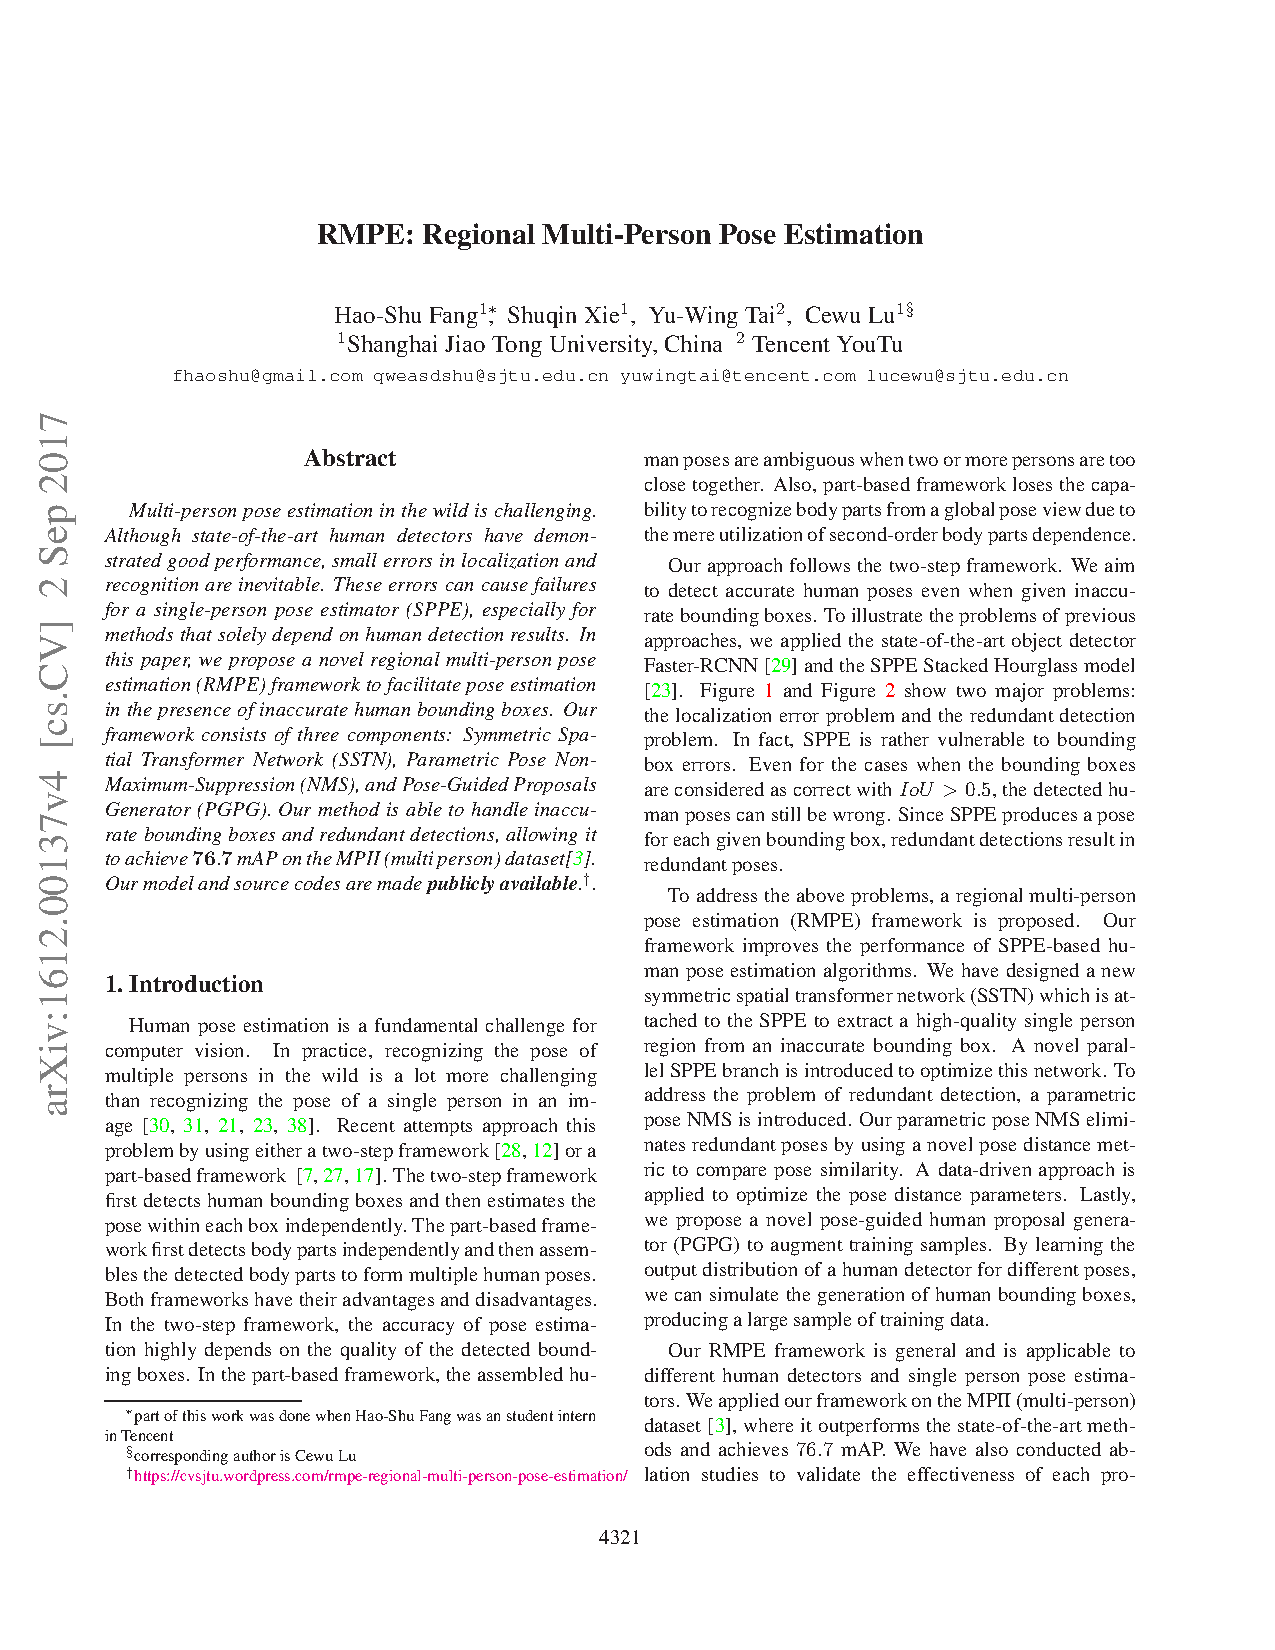
\includepdf[pages={1-}]{RMPE.pdf}
\end{appendix}

\end{document}
